\documentclass[a4paper, 12pt]{article}
\usepackage[utf8]{inputenc}
\usepackage[T1, T2A]{fontenc}
\usepackage[a4paper, top=2cm, bottom=2cm, left=1cm, right=1cm, marginparwidth=1.75cm]{geometry}
\usepackage{graphicx}
\usepackage{amsmath}
\usepackage{indentfirst}
\usepackage[english, russian]{babel}
\usepackage[section,above,below]{placeins}
\usepackage[noend]{algorithmic}

\begin{document}

\noindent 

\noindent 

\noindent 

\noindent МИНИСТЕРСТВО ОБРАЗОВАНИЯ И НАУКИ РОССИЙСКОЙ ФЕДЕРАЦИИ

\noindent Федеральное государственное бюджетное образовательное учреждение высшего образования

\noindent \textbf{«КУБАНСКИЙ ГОСУДАРСТВЕННЫЙ УНИВЕРСИТЕТ»         (ФГБОУ ВО «КубГУ»)}

\noindent 

\noindent \textbf{Кафедра математических и компьютерных методов}

\noindent 

\noindent 

\noindent 

\noindent 

\noindent 

\noindent \textbf{ДИПЛОМНАЯ РАБОТА}

\noindent \textbf{}

\noindent \textbf{Устойчивый алгоритм аппроксимации в гильбертовом пространстве по любой независимой системе функций}

\noindent

\noindent
  
\noindent 

\noindent 

\noindent Работу выполнил\underbar{                                                                  }Д. А. Пасько

\noindent (подпись, дата)

\noindent 

\noindent Факультет\underbar{ математики и компьютерных наук                  }курс\underbar{    3~~    ~~~~} 

\noindent Направление\underbar{ 02.03.01 математика и компьютерные науки                   ~}                                 

\noindent 

\noindent Научный руководитель                                                                                                              доцент кафедры МКМ,

\noindent канд. физ.-мат. наук\underbar{                                                             }А. А. Свидлов 

\noindent (подпись, дата)

\noindent Нормоконтролер

\noindent ст. лаборант\underbar{                                                                           }Ю. А. Кравченко\underbar{}

\noindent (подпись, дата)

\noindent 

\noindent 

\noindent 

\noindent 

\noindent Краснодар 2018

\section{ВВЕДЕНИЕ}

Аппроксимация функций -- одно из самых востребованных направлений прикладной математики. Задача аппроксимации считается полностью решённой в сепарабельных гильбертовых пространствах, однако ввиду ограничений, налагаемых компьютерной арифметикой, современная математическая теория не может быть применима на практике во всей полноте. Задачи из многих математических областей при численном решении сталкиваются с существенными ограничениями; в теории приближений таким ограничением является неустойчивость аппроксимации. Для обхода этого ограничения требуется использовать специальные алгоритмы, учитывающие как особенности компьютерной реализации, так и естественные требования к точности и производительности.

В этой работе описан алгоритм сложности $O(n^4)$, реализующий устойчивую аппроксимацию. Также описываются многие особенности численной аппроксимации, которые пришлось учитывать при разработке этого алгоритма.

\section{Обозначения}

$\left(x,y\right)$ -- точка на плоскости с координатами $x,y$;
$x=\left(x_1,\dots ,x_n\right)$ -- вектор из пространства $R^n$;
$x^m=\left(x_1,\dots ,x_m\right)$ -- $m$-мерный вектор;
$\Delta =\sum^n_{i=1}{\dfrac{{\partial }^2}{{{\partial }^2x}_i}}$ -- оператор Лапласа;
$L\left(f_1,\dots ,f_m\right)=\sum^m_{i=1}{{\alpha }_if_i}$, ${\alpha }_i\in \ R$ -- множество всевозможных линейных комбинаций элементов $f_1,\dots ,f_m$(линейная оболочка);
$\varphi =\varphi \left(x\right)$ -- граничная функция;
$D_{c_i}=\frac{\partial }{{\partial c}_i}$ -- частная производная по аргументу $c_i$;
$Q$ -- область на плоскости либо некоторое произвольное множество;
${L}_2\left(\partial Q\right)$ -- пространство функций, определённых на кривой $\partial Q$ и интегрируемых с квадратом в смысле Лебега;
${({\alpha }_n,\alpha }_m)$ -- скалярное произведение функций в определённом пространстве ${{({\alpha }_n,\alpha }_m)}_{{\ L}_2\left(\partial Q\right)}=\oint_{\partial Q}{{{\alpha }_n\left(x\right)\alpha }_m\left(x\right)dl}$ -- скалярное произведение функций${({\alpha }_n,\alpha }_m)\in {L}_2\left(\partial Q\right)$;
${Q^+=R}^2\backslash (Q\cup \partial Q)$;
$\varepsilon$ -- некоторое очень малое число, большее нуля;
а. п. -- аналитическое продолжение функции на всю плоскость, используемое для упрощения программирования этой функции.

\section{Общие сведения о задаче аппроксимации}

В общем случае задача аппроксимации состоит в следующем: требуется максимально точно приблизить некоторый элемент $x\in \textrm{Х}$  элементами пространства $F\subset \textrm{Х},\ x\notin F$.
Качество приближения оценивается по тому, насколько малым оказывается расстояние от элемента $x\in \textrm{Х}$ до элемента $u\in F$, наиболее близкого к $x$ в заданной метрике; само же это расстояние выражается формулой:
\begin{equation} \rho \left(x,F\right)={\mathrm{inf}}_{u\in F}\left\|x-u\right\|.\end{equation} 

Если для какого-то $u_0\in F$ инфинум достигается, то $u_0$ называется элементом наилучшего приближения. Этот элемент и представляет из себя цель поиска. Далее будем рассматривать только такие случаи, когда элементы наилучшего приближения существуют.

На практике аппроксимация происходит исключительно элементами конечномерных пространств.
Так как в конечномерных пространствах имеются базисы, можно выбрать любой из них и искать элемент наилучшего приближения как линейную комбинацию элементов базиса.
Сразу же ставятся вопросы: 1) найдётся ли на подпространстве элемент наилучшего приближения и 2) будет ли он единственным?
На оба вопроса в самых распространённых случаях ответы положительны; во-первых, в конечномерном подпространстве элемент наилучшего приближения однозначно существует (\cite{9korn, 10ax}); во-вторых, при нахождении решения обычно работают с функциями из строго нормированных пространств (включая ${\ L}_2\left(Q\right)$, где $Q$ -- компакты либо поверхности в многомерном евклидовом пространстве), а из строгой нормированности следует единственность элемента наилучшего приближения; более того, пространство ${\ L}_2\left(Q\right)$ является гильбертовым, а потому наилучшим приближением элемента $x\in $ ${\ L}_2\left(Q\right)$ является его проекция на линейную оболочку $L\left(f_1,\dots ,f_m\right)$ исходного множества. Таким образом, задача аппроксимации сводится к задаче минимизации функционала
\begin{equation}F\left(c\right)={\left\|\varphi -\sum^N_{m=1}{c_m}{\alpha }_m\right\|}_{{\ L}_2\left(Q\right)}\to \mathrm{min},\\\end{equation} 
где $\varphi \in $ ${\ L}_2\left(Q\right)$ -- аппроксимируемая функция, ${\alpha }_m\in {\ L}_2\left(Q\right)\mathrm{\ },m=1,\dots ,N$ -- базис подпространства, в котором ищется элемент наилучшего приближения.

Решим задачу аппроксимации аналитически. Так как пространство ${\ L}_2\left(Q\right)$ -- гильбертово, то норма в нём выражается через скалярное произведение:

\begin{multline}{\left\|\varphi -\sum^N_{m=1}{c_m}{\alpha }_m\right\|}_{{\ L}_2\left(Q\right)}=\sqrt{{\left(\varphi -\sum^N_{m=1}{c_m}{\alpha }_m,\varphi -\sum^N_{m=1}{c_m}{\alpha }_m\right)}_{{\ L}_2\left(Q\right)}}=\\ 
\sqrt{\left(\varphi ,\varphi \right)-2\sum^N_{m=1}{c_m}\left(\varphi ,{\alpha }_m\right)+\sum^N_{n=1}{c_n}\sum^N_{m=1}{c_m}{({\alpha }_n,\alpha }_m)}\end{multline} 

Так как норма является неотрицательной по определению, то предыдущее выражение можно возвести в квадрат без риска потерять решения или обрести новые:

\begin{multline}{\left\|\varphi -\sum^N_{m=1}{c_m}{\alpha }_m\right\|}^2_{{\ L}_2\left(Q\right)}={\left(\varphi ,\varphi \right)}_{{\ L}_2\left(Q\right)}-2\sum^N_{m=1}{c_m}{\left(\varphi ,{\alpha }_m\right)}_{{\ L}_2\left(Q\right)}+\sum^N_{n=1}{c_n}\sum^N_{m=1}{c_m}{{({\alpha }_n,\alpha }_m)}_{{\ L}_2\left(Q\right)}=\\
    {\left(\varphi ,\varphi \right)}_{{\ L}_2\left(Q\right)}-2\sum^N_{m=1}{c_m}{\left(\varphi ,{\alpha }_m\right)}_{{\ L}_2\left(Q\right)}+\left(c_1,c_2,\dots ,c_N\right)\left( \begin{array}{ccc}
{{({\alpha }_1,\alpha }_1)}_{{\ L}_2\left(Q\right)} & \cdots  & {{({\alpha }_1,\alpha }_N)}_{{\ L}_2\left(Q\right)} \\ 
\vdots  & \ddots  & \vdots  \\ 
{{({\alpha }_N,\alpha }_1)}_{{\ L}_2\left(Q\right)} & \cdots  & {{({\alpha }_N,\alpha }_N)}_{{\ L}_2\left(Q\right)} \end{array}
\right)\left( \begin{array}{c}
c_1 \\ 
\vdots  \\ 
c_N \end{array}
\right),\end{multline} 
причём возникшая матрица Грама является невырожденной, если система функций ${\alpha }_m\in {\ L}_2\left(Q\right)$ линейно независима; следовательно, аппроксимировать имеет смысл только по линейно независимым система (иначе получится неоднозначное решение).

Получено выражение квадратичного функционала. Вычислим стационарные точки этого функционала из системы:
\begin{equation}D_{c_i}F\left(c\right)=0,\ i=1,\ 2,\ \dots ,\ N,\\\end{equation} 
где
\begin{multline}D_{c_i}F\left(c\right)=D_{c_i}\left({\left(\varphi,\varphi\right)}_{{\ L}_2\left(Q\right)}-2\sum^N_{m=1}{c_m}{\left(\varphi,\alpha_m\right)}_{{\ L}_2\left(Q\right)}+\sum^N_{n=1}{c_n}\sum^N_{m=1}{c_m}{(\alpha_n,\alpha}_m)\right)=\\
-2{\left(\varphi,\alpha_i\right)}_{{\ L}_2\left(Q\right)}+\sum^N_{n=1}{D_{c_i}\left(c_n\right)}\sum^N_{m=1}{c_m}{{(\alpha_n,\alpha}_m)}_{{\ L}_2\left(Q\right)}+\sum^N_{n=1}{c_n}D_{c_i}\sum^N_{m=1}{c_m}{{(\alpha_n,\alpha}_m)}_{{\ L}_2\left(Q\right)}=\\
-2{\left(\varphi,\alpha_i\right)}_{{\ L}_2\left(Q\right)}+\sum^N_{m=1}{c_m}{{(\alpha_i,\alpha}_m)}_{{\ L}_2\left(Q\right)}+\sum^N_{n=1}{c_n}{{(\alpha_n,\alpha}_i)}_{{\ L}_2\left(Q\right)}=\\
2\left(\sum^N_{m=1}{c_m}{{(\alpha_i,\alpha}_m)}_{{\ L}_2\left(Q\right)}-{\left(\varphi,\alpha_i\right)}_{{\ L}_2\left(Q\right)}\right)\end{multline} 

Такая система сводится к виду
\begin{equation}\Gamma c=\left( \begin{array}{c}
{\left(\varphi ,{\alpha }_1\right)}_{{\ L}_2\left(\partial Q\right)} \\ 
\vdots  \\ 
{\left(\varphi ,{\alpha }_N\right)}_{{\ L}_2\left(\partial Q\right)} \end{array}
\right),\\\end{equation} 
где $c=\left(c_1,c_2,\dots ,c_N\right)$, $\Gamma $ -- матрица Грама нашей системы. Так как эта матрица является невырожденной, система имеет единственное решение; поскольку второй дифференциал функции$\ F\left(c\right)$ является положительно определённой квадратичной формой с той же матрицей Грама, то в точке решения нашей системы функция $F\left(c\right)$ действительно имеет минимум. Сама же погрешность аппроксимации равна:

\begin{multline}\rho \left(\sum^N_{m=1}{c_m}{\alpha }_m,\varphi \right)={\left\|\varphi -\sum^N_{m=1}{c_m}{\alpha }_m\right\|}_{{\ L}_2\left(Q\right)}=\sqrt{\oint_Q{{\left(\sum^N_{m=1}{c_m}{\alpha }_m-\varphi \right)}^2dl}}\ =\\
    {\left({\left(\varphi ,\varphi \right)}_{{\ L}_2\left(Q\right)}-2\sum^N_{m=1}{c_m}{\left(\varphi ,{\alpha }_m\right)}_{{\ L}_2\left(Q\right)}+\left(c_1,c_2,\dots ,c_N\right)\left( \begin{array}{ccc}
{{({\alpha }_1,\alpha }_1)}_{{\ L}_2\left(Q\right)} & \cdots  & {{({\alpha }_1,\alpha }_N)}_{{\ L}_2\left(Q\right)} \\ 
\vdots  & \ddots  & \vdots  \\ 
{{({\alpha }_N,\alpha }_1)}_{{\ L}_2\left(Q\right)} & \cdots  & {{({\alpha }_N,\alpha }_N)}_{{\ L}_2\left(Q\right)} \end{array}
\right)\left( \begin{array}{c}
c_1 \\ 
\vdots  \\ 
c_N \end{array}
\right)\right)}^{\frac{1}{2}}=\\
{\left({\left(\varphi ,\varphi \right)}_{{\ L}_2\left(Q\right)}-2\left(c_1,c_2,\dots ,c_N\right)\left( \begin{array}{c}
{\left(\varphi ,{\alpha }_1\right)}_{{\ L}_2\left(Q\right)} \\ 
\vdots  \\ 
{\left(\varphi ,{\alpha }_N\right)}_{{\ L}_2\left(Q\right)} \end{array}
\right)+\left(c_1,c_2,\dots ,c_N\right)\left( \begin{array}{c}
{\left(\varphi ,{\alpha }_1\right)}_{{\ L}_2\left(Q\right)} \\ 
\vdots  \\ 
{\left(\varphi ,{\alpha }_N\right)}_{{\ L}_2\left(Q\right)} \end{array}
\right)\right)}^{\frac{1}{2}}=\\
{\left({\left(\varphi ,\varphi \right)}_{{\ L}_2\left(Q\right)}-\left(c_1,c_2,\dots ,c_N\right)\left( \begin{array}{c}
{\left(\varphi ,{\alpha }_1\right)}_{{\ L}_2\left(Q\right)} \\ 
\vdots \\ 
{\left(\varphi ,{\alpha }_N\right)}_{{\ L}_2\left(Q\right)} \end{array}
\right)\right)}^{\frac{1}{2}}.\end{multline} 

На этом задача аппроксимации в гильбертовом пространстве считается теоретически решённой. На данный момент мы условились брать только линейно независимые системы функций, иначе задача не решится ввиду вырожденной матрицы Грама. Также крайне желательно, чтобы система ${\alpha }_m\in {\ L}_2\left(Q\right)$ обладала свойством полноты; полная система сможет обеспечивать безграничное возрастание точности аппроксимации при своём расширении. Система из множества $S\subset {\ L}_2\left(Q\right)$ является полной, если для любого элемента$\ f$ из ${\ L}_2\left(Q\right)$ и для всякой наперёд заданной точности найдётся комбинация элементов из $S$, обеспечивающая данную точность; для практики полнота системы означает, что с ростом числа функций точность всегда будет улучшаться:
\begin{equation}\left\|f-\sum_{s\in S_n}{c_s\left(f\right)s}\right\|\to 0,\ n\to \infty ,\ S_1\subset S_2\subset \dots \subset S_n\subset \dots \subset S.\end{equation} 
Если же система функций не будет полной, мы никакими способами не сможем осуществить с её помощью приближение лучшее, чем некоторое. Но на практике мы сталкиваемся с той же самой проблемой даже при работе с полными системами: ошибки округлений и заведомо неточные вычисления приводят к тому, что аппроксимация становится крайне неустойчивой, поэтому теряются гарантии эффективного использования теории на практике. Цель следующего изложения -- указать причины неустойчивости и предложить алгоритм, исключающий её.


\section{Причины неустойчивости аппроксимации и примеры неустойчивости для распространённых систем функций}

Наибольший вклад в неустойчивость аппроксимации вносят три причины:

\begin{enumerate}
\item  Скалярные произведения, заполняющие СЛАУ, обычно представляются конечными суммами или интегралами; при этом это могут быть интегралы по сложным областям или поверхностям или интегралы от функций, которые сами задаются интегралами; в таком случае погрешности квадратурных формул накапливаются и приводят к тому, что исходная СЛАУ несколько отличается от истинной, что негативно сказывается на решении задачи. Даже если удаётся подобрать реализуемый способ интегрирования, часто попытки повысить точность существенно увеличивают время вычислений.

\item  Матрица Грамма для любой системы функций является плохо обусловленной по определению, причём число обусловленности быстро растёт с увеличением размерности, из-за чего даже малые отклонения в элементах системы (которые будут иметь место хотя бы по причине пункта 1) приводят к неточным решениям.

\item  Огромную роль играют погрешности округления при суммировании больших и маленьких чисел, делении и умножении; эти погрешности заметны при вычислении интегралов, решении СЛАУ и даже при замене координат (для получения системы, ортогональной на произвольном отрезке). Позднее будет показано, что при плохо обусловленной матрице системы даже итерационные методы не способны из-за ошибок округления приблизиться к истинному решению ближе некоторого расстояния. Комбинация пунктов 1) и 3) приводит к тому, что даже аппроксимация по  ортогональным системам обладает неустойчивостью при достаточно большом числе функций.
\end{enumerate}

Далее рассматривается аппроксимация для наиболее распространённых систем функций:

\begin{enumerate}
\item  Мономы ($1,\ x,{\ x}^2,{\ x}^3,\dots $). Традиционный пример полной системы. Матрица Грамма для мономов есть так называемая матрица Гильберта -- классический пример плохо обусловленной матрицы. Из-за плохой обусловленности неустойчивость возникает выраженная, хотя на первых порах приближение происходит лучше, чем по другим системам. Время и погрешности вычислений можно уменьшить, если реализовать мономы в виде некоторого класса с реализацией схемы Горнера.

\item  Тригонометрические полиномы ($1/2,\ {\sin x},{\cos x},{\sin\mathrm{2}x},\dots$). Распространённая ортогональная система, часто используемая при аппроксимации колебаний. Основной недостаток -- медленная сходимость: иногда для приличной аппроксимации приходится использовать несколько сотен функций.

\item  Многочлены Лежандра ($P_0=1, P_1=x, P_{n+1}=\frac{2n+1}{n+1}x P_n-\frac{n}{n+1}P_{n-1}$). Результат ортогонализации системы из пункта 1, за счёт ортогональности эта система более устойчива, однако численная реализация для большой размерности из-за рекурсии приводит к сильно заметным временным затратам.

\item  Экспоненты ($1,\ e^x,\ e^{2x},\dots $). Неортогональная система, обладает медленной сходимостью и сильной неустойчивостью за счёт быстрого роста экспоненты и больших коэффициентов в СЛАУ.

\item  Система Хаара. Ортогональная система, используется для аппроксимации шумов, обладает соразмерной сходимостью с системой 2, но неустойчивостью почти как у системы 4.
\end{enumerate}

Неустойчивость каждой системы выражается по-своему. На следующем графике (Рис. 1) показана зависимость погрешности аппроксимации от числа функций по разным системам. Приближается функция $y=-e^{x/2}+\left|x\right|{\cos \left(x\right)\ }$ на отрезке $\left[-3,1\right]$. На оси Х показано количество функций, на оси Y -- десятичный логарифм от погрешности. Все СЛАУ решались методом Гаусса с выбором максимального элемента, интегралы в СЛАУ считаются по формулам Гаусса-Кронрода при 61 точках.

\begin{figure}[h!]
    \noindent\centering{
    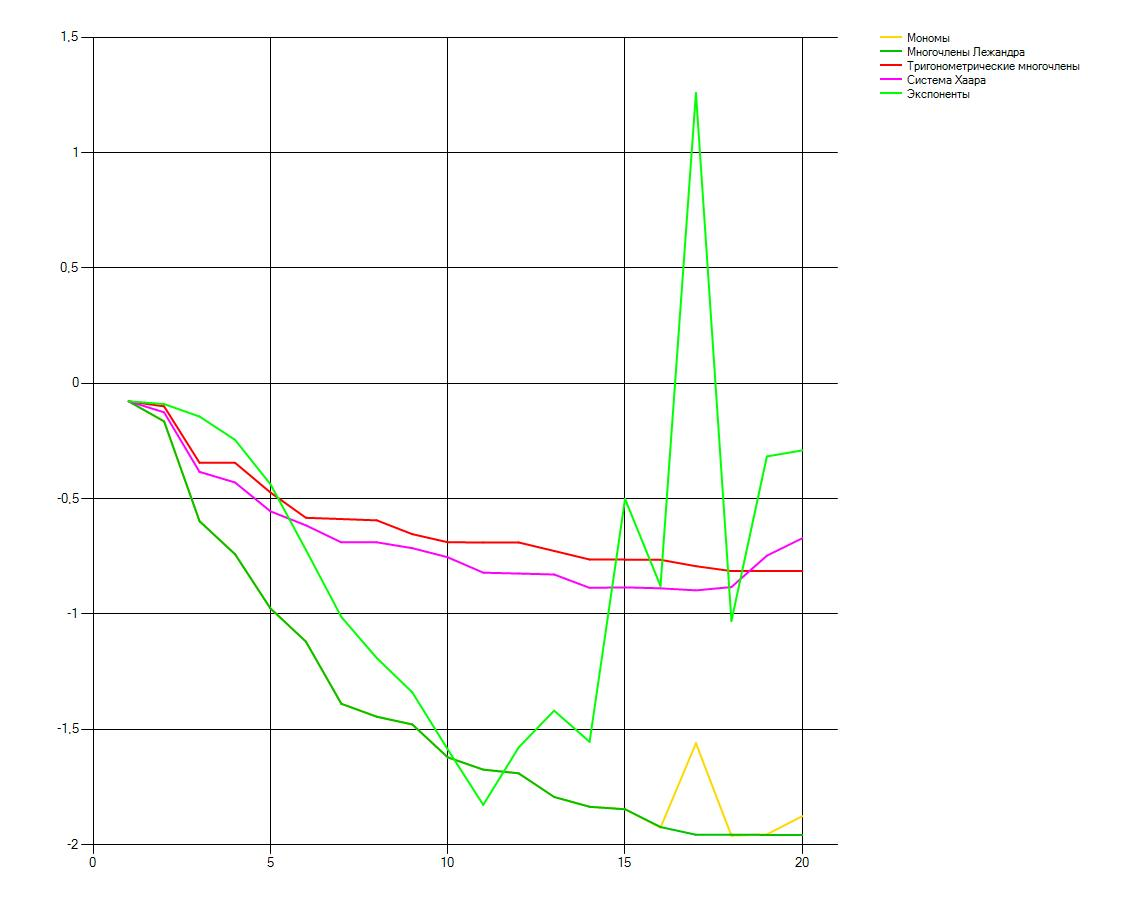
\includegraphics[width=\linewidth]{1.png}
  }
    \caption{Погрешность аппроксимации функции $y=-e^{x/2}+|x|\cos(x), x\in[-3;1]$ разными системами при разном количестве функций в системах}
    \label{figCurves}
\end{figure}     

Как видно из Рис. 1, системы мономов и Хаара начали показываться неустойчивость (скачки) при 16-18 функциях, система по экспонентам неустойчива уже с 11 функций и на 17-й имеет сильный скачок. Относительно аппроксимации получены следующие данные:

\begin{enumerate}
\item  Для системы мономов наилучшая аппроксимация равна 0,0109251874472286 при числе функций 18

\item  Для системы полиномов Лежандра наилучшая аппроксимация равна 0,0110161134996089 при числе функций 19

\item  Для ортонормированной системы тригонометрических полиномов наилучшая аппроксимация равна 0,153425238548837 при числе функций 20

\item  Для системы Хаара наилучшая аппроксимация равна 0,12656928280189 при числе функций 17

\item  Для системы экспонент наилучшая аппроксимация равна 0,0148738092936054 при числе функций 11
\end{enumerate}

Систему по экспонентам использовать нет смысла из-за сильной неустойчивости и очень медленного роста аппроксимации; многочлены Лежандра не могут быть использованы при больших размерностях из-за больших затрат по времени. Остальные системы могут быть полезны, если уметь их корректировать. Увеличим число функций и пересмотрим результат (Рис. 2).

\begin{figure}[h!]
    \noindent\centering{
    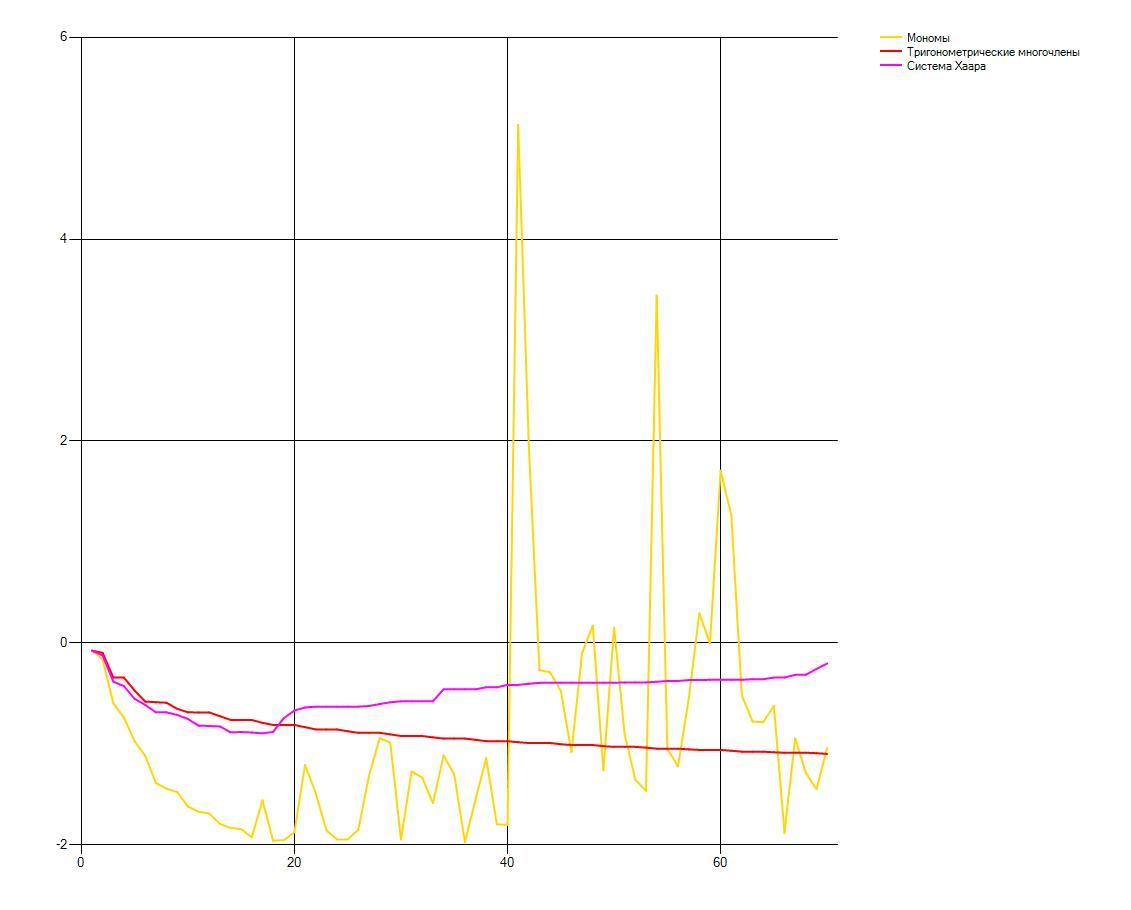
\includegraphics[width=\linewidth]{2.png}
  }
    \caption{Аппроксимация при тех же условиях, но с увеличенным числом функций в системах}
    \label{figCurves}
\end{figure}

Погрешность по системе Хаара продолжила возрастать, погрешность по системе мономов при больше чем 20 функция целиком состоит из неустойчивости. При этом наилучшие результаты, можно сказать, почти не изменились:

\begin{enumerate}
\item  Для системы мономов наилучшая аппроксимация равна 0,0106044647958804 при числе функций 36

\item  Для ортонормированной системы тригонометрических полиномов наилучшая аппроксимация равна 0,0791846313802487 при числе функций 70

\item  Для системы Хаара наилучшая аппроксимация равна 0,12656928280189 при числе функций 17
\end{enumerate}

Дальнейшее увеличение числа функций приведёт к неустойчивости тригонометрической системы (Рис. 3).

\begin{figure}[h!]
    \noindent\centering{
    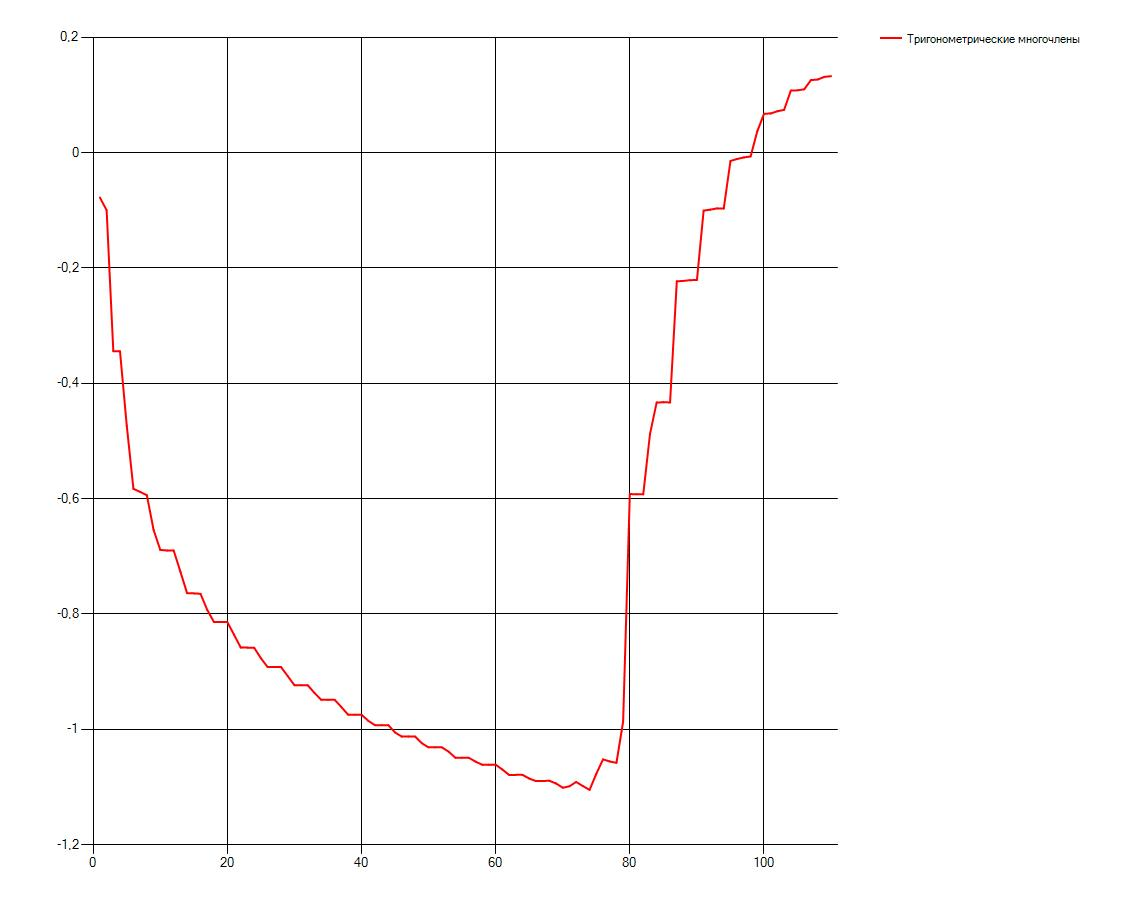
\includegraphics[width=\linewidth]{3.png}
  }
    \caption{Те же условия аппроксимации, ещё больше функций в системах}
    \label{figCurves}
\end{figure}

На Рис. 4 изображены аналогичные графики для функции $y=e^{x/\left|x\right|+1}$ на отрезке $\left[0,5\right]$ (далее часто будет проводиться аппроксимация именно этой функции на этом отрезке, дабы сравнивать результаты в равных условиях).

\begin{figure}[h!]
    \noindent\centering{
    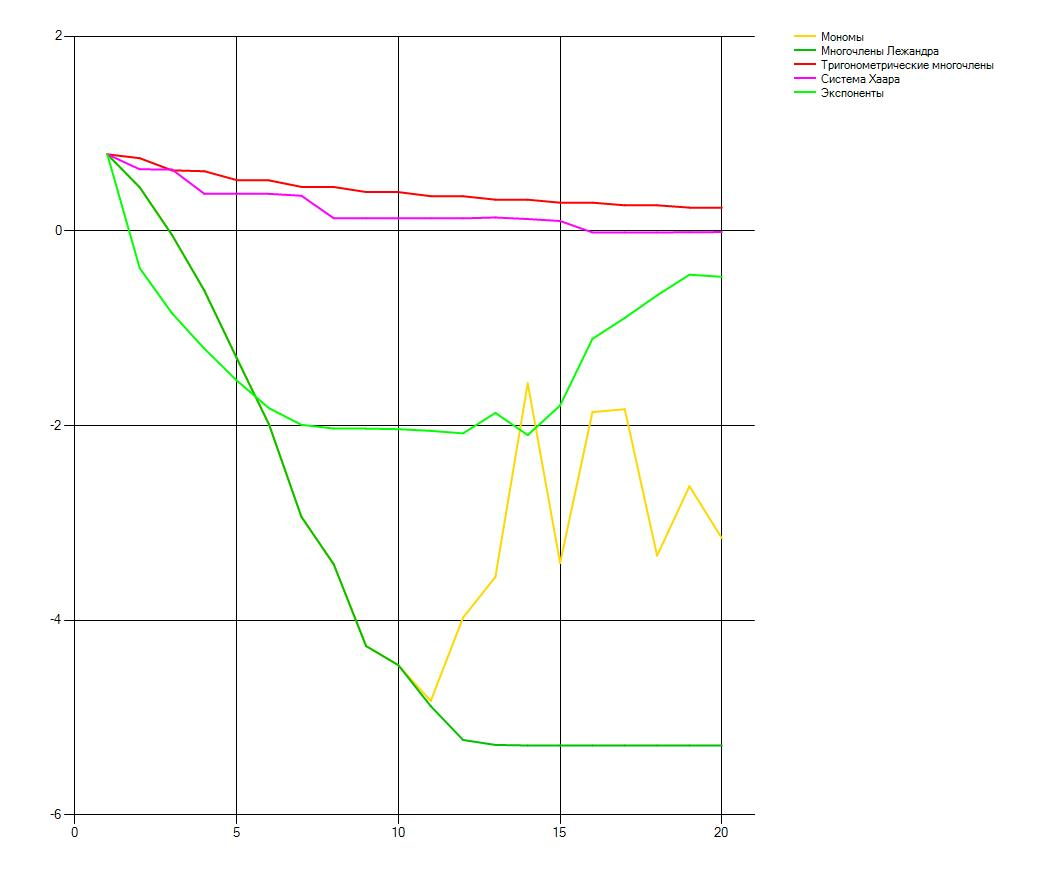
\includegraphics[width=\linewidth]{4.png}
  }
    \caption{Погрешность аппроксимации функции $y=e^{x/\left|x\right|+1}, x\in[0;5]$ разными системами при разном количестве функций в системах}
    \label{figCurves}
\end{figure}

\begin{figure}[h!]
    \noindent\centering{
    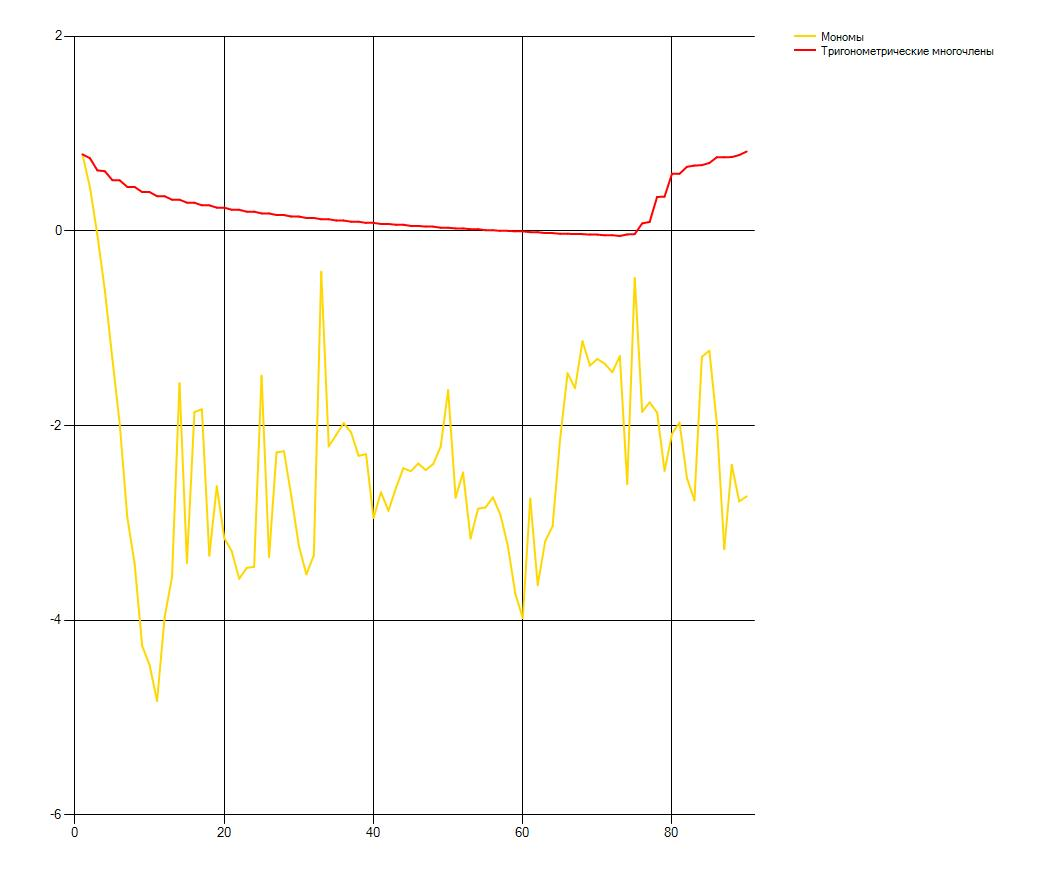
\includegraphics[width=\linewidth]{5.png}
  }
    \caption{Погрешность аппроксимации функции $y=e^{x/\left|x\right|+1}, x\in[0;5]$ разными системами при разном количестве функций в системах (при большем количестве функций)}
    \label{figCurves}
\end{figure}

\section{Попытки обойти неустойчивость, меняя точность интегрирования и комбинируя разные методы решения СЛАУ}

Если при интегрировании использовать квадратуры Гаусса-Кронрода при 15 точках (а не 61), неустойчивость в предыдущем случае становится намного выраженнее и наступает раньше (Рис. 6).

\begin{figure}[h!]
    \noindent\centering{
    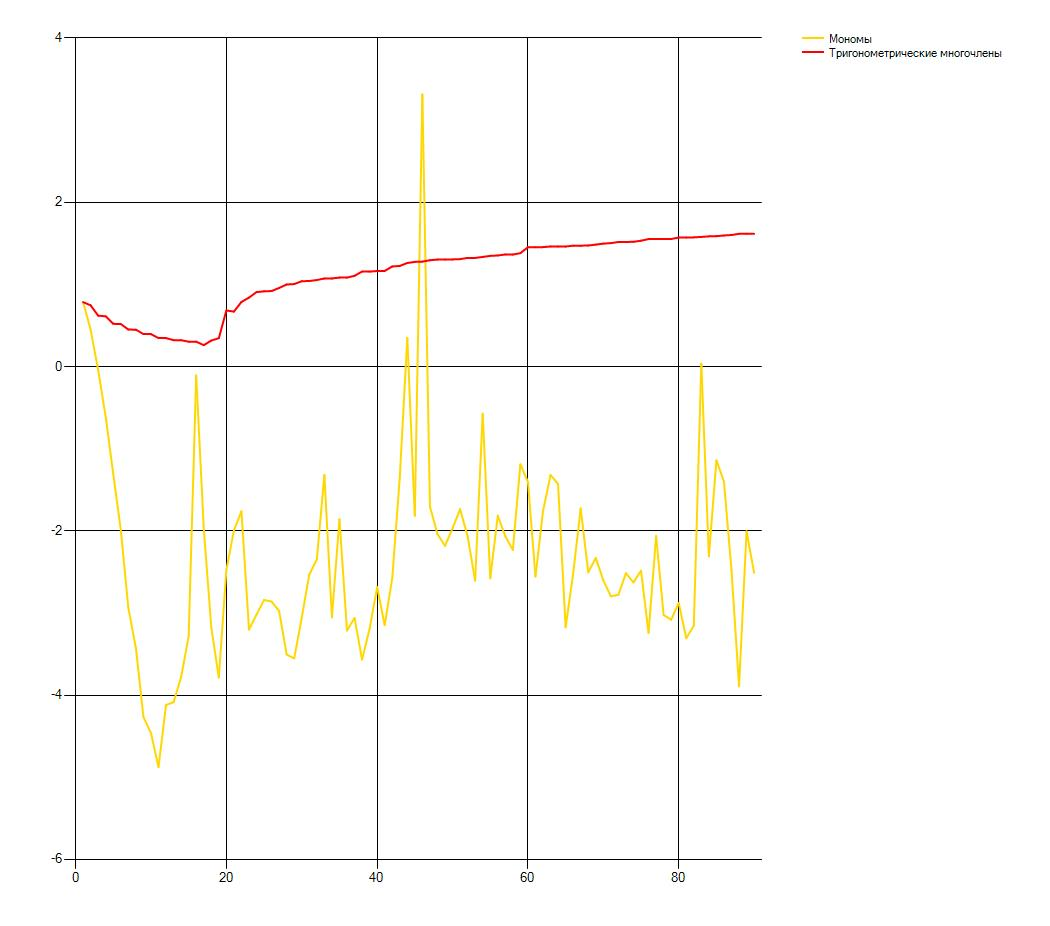
\includegraphics[width=\linewidth]{6.png}
  }
    \caption{Погрешность аппроксимации функции $y=e^{x/\left|x\right|+1}, x\in[0;5]$ разными системами при разном количестве функций в системах (при менее точном интегрировании)}
    \label{figCurves}
\end{figure}

Вывод: увеличение точности подсчёта интегралов в СЛАУ «сглаживает» неустойчивость, но полностью не устраняет её. Поэтому при заполнении СЛАУ следует добиться некоторого баланса между точностью и временем вычислений; на мой взгляд, квадратуры Гаусса-Кронрода при 31, 51, 61 точках наиболее оптимальны в этом случае. Считая проблему интегрирования вполне решённой, попытаемся решить другие проблемы.

Посмотрим, «сгладится» ли аппроксимация, если попытаться решать СЛАУ точнее. Метод Холецкого в данном случае, как оказывается, не поможет, поскольку плохая обусловленность матрицы Грама и ошибки округления делают её не положительно определённой при числе функций около 15 (в этом случае в методе Холецкого появляются корни из отрицательных чисел). Чтобы в этом убедиться, посчитаем определители диагональных миноров матрицы Гильберта для отрезка $\left[0,2\right]$ и числа функций 20; результаты оформлены в таблицу Рис. 7.

\begin{figure}[h!]
    \noindent\centering{
    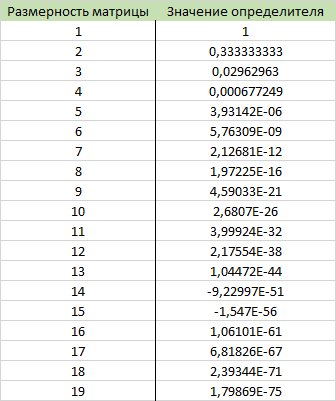
\includegraphics[width=9cm]{61.png}
  }
    \caption{Зависимость определителя матрицы Гильберта от размерности матрицы ($A_{i,j} =\int_h x^{i+j-2} dx,  h=[0,2], i,j=1,\dots n$, $A$ -- матрица Гильберта, $n$ -- её размерность)}
    \label{figCurves}
\end{figure}

Если взять другой отрезок, результаты изменятся по модулю, но всё равно сохранят тенденцию (Рис. 8).
 \begin{figure}[h!]
    \noindent\centering{
    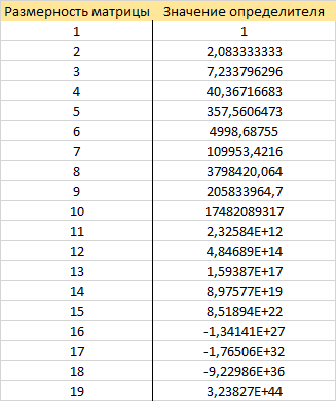
\includegraphics[width=9cm]{62.png}
  }
    \caption{Аналогичная таблица при $h=[-1,4]$}
    \label{figCurves}
\end{figure}
Описанную тенденцию можно изобразить визуально (Рис. 9).

\begin{figure}[h!]
    \noindent\centering{
    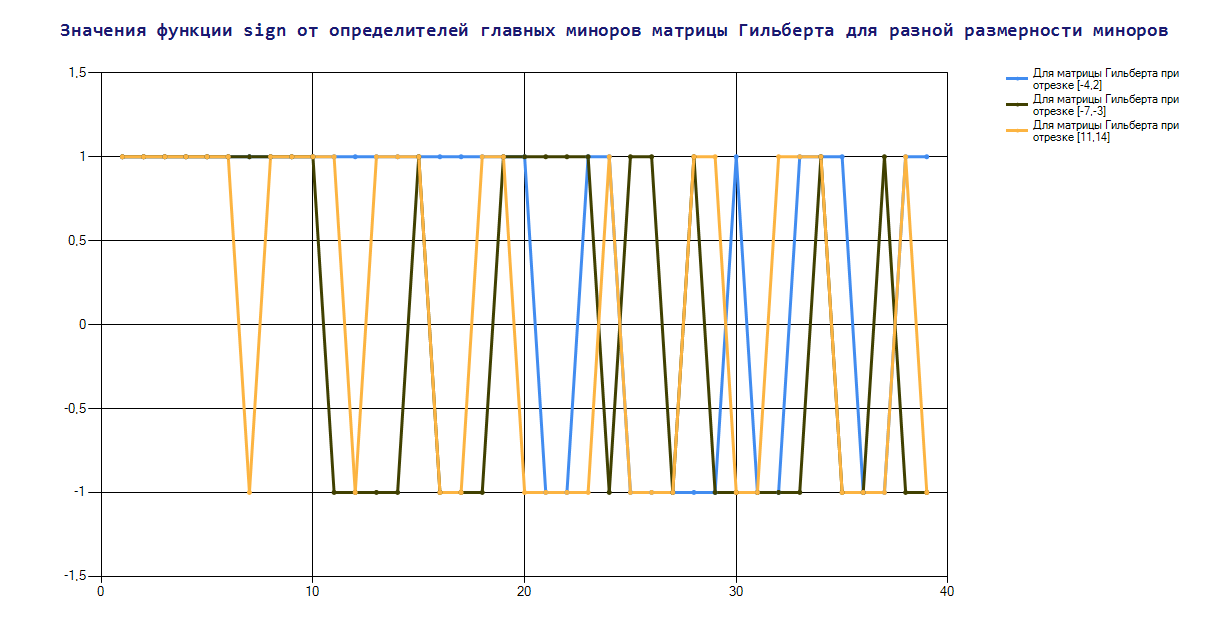
\includegraphics[width=\linewidth]{7.png}
  }
    \caption{Матрица Грама при большой размерности численно перестаёт быть положительно определённой}
    \label{figCurves}
\end{figure}

Поскольку метод Холецкого использовать нельзя, но метод Гаусса сам по себе является вполне эффективным, попробуем улучшить решение СЛАУ, используя результат метода Гаусса как начальное приближение в методе наискорейшего спуска, выведенного специально для задач минимизации квадратичных функционалов; напомню, что этот метод является итерационным и может быть выражен формулой
\begin{equation}x^{k+1}=x^k-\frac{\left(r^k,r^k\right)}{\left(Ar^k,r^k\right)}r^k,x^0-\textrm{л}\textrm{ю}\textrm{б}\textrm{о}\textrm{й}\ \textrm{в}\textrm{е}\textrm{к}\textrm{т}\textrm{о}\textrm{р}\\\end{equation} 
где $r^k=Ax^k-b$, $b$ -- свободный вектор СЛАУ, $A$ -- матрица СЛАУ; для ускорения сходимости вектор $x^0$ желательно брать достаточно близким к истинному решению, что мы и сделаем, взяв за $x_0$ результат решения СЛАУ методом Гаусса. Как показывают тесты, этот метод для конкретно задачи аппроксимации сходится не всегда, что, возможно, обусловлено нарушением положительной определённости матрицы Грамма при большой размерности; по этой причине количество итераций в методе будет ограничено заранее заданным значением и если после очередной итерации невязка решения СЛАУ возрастёт, метод вернёт прежнее значение и завершится принудительно. Для удобства назовём этот метод {\it гибридным}. Аппроксимируя, как и предыдущем случае, функцию $y=e^{x/\left|x\right|+1}$ на отрезке $\left[0,5\right]$, видим (Рис. 10), что неустойчивость слегка сгладилась (для системы экспонент).

\begin{figure}[h!]
    \noindent\centering{
    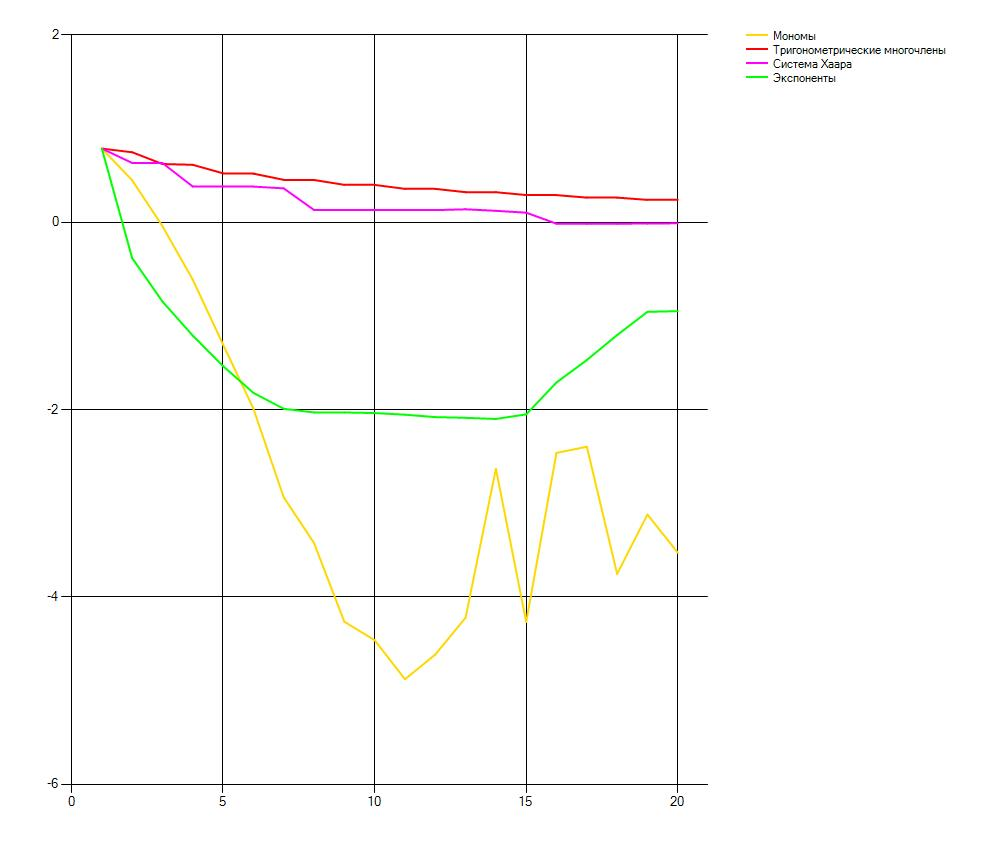
\includegraphics[width=\linewidth]{8.png}
  }
    \caption{Погрешность аппроксимации функции $y=e^{x/\left|x\right|+1}, x\in[0;5]$ разными системами при разном количестве функций в системах (при гибридном способе решения СЛАУ)}
    \label{figCurves}
\end{figure}
Однако увеличение числа функций по-прежнему приводит к сильным скачкам (Рис. 11).

\begin{figure}[h!]
    \noindent\centering{
    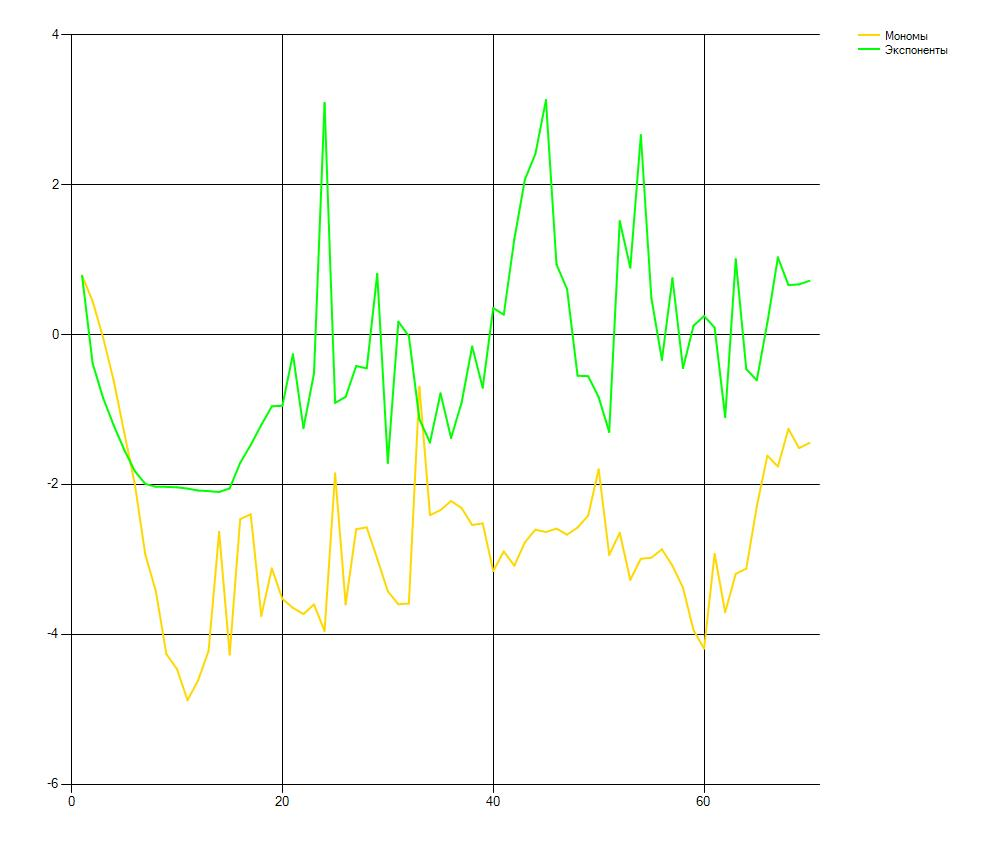
\includegraphics[width=\linewidth]{9.png}
  }
    \caption{Погрешность аппроксимации функции $y=e^{x/\left|x\right|+1}, x\in[0;5]$ разными системами при разном количестве функций в системах (гибридный метод не решает проблему неустойчивости)}
    \label{figCurves}
\end{figure}
Это связано с тем, что для систем большой размерности невязка при использовании метода наискорейшего спуска начинает возрастать уже с 1-3 шага, либо изначально очень велика и не меняется, так что польза от добавления наискорейшего спуска сомнительна.

Существует алгоритм уточнения решения (\cite{algol}), выражающийся формулой
$$x^{s+1}=x^s+A^{-1}(b-Ax^s), s \geq 0, x^0 \text{ -- любой вектор}$$
но и он не приносит заметной пользы, поскольку матрица Грама плохо обусловлена и к тому же численно не положительно определённая.

Дальнейшие попытки улучшить решение СЛАУ заведомо бесполезны, поскольку погрешности вычислений и квадратур вместе с плохой обусловленностью матриц не дадут достигнуть более точного решения, а более точное решение само по себе будет лишь приближённым решением задачи аппроксимации. Действительно, следующие графики (Рис. 12, Рис. 13) показывают, что между погрешностью аппроксимации и погрешностью решения СЛАУ корреляция не обязательна, поскольку даже при больших невязках погрешность может оставаться малой и далеко не всегда рост невязок означает рост погрешности. Кроме того, графики показывают, как быстро растут невязки системы, несмотря на все старания решать её точно.

\begin{figure}[h!]
    \noindent\centering{
    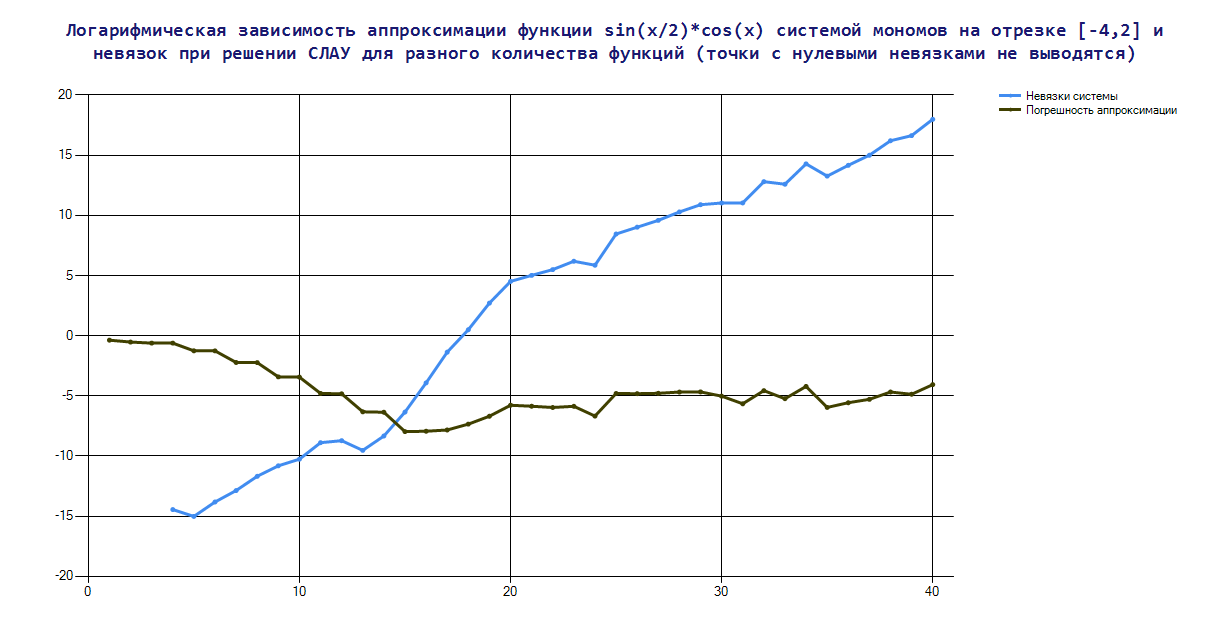
\includegraphics[width=\linewidth]{10.png}
  }
    \caption{Между невязкой и погрешностью нет заметной связи}
    \label{figCurves}
\end{figure}

\begin{figure}[h!]
    \noindent\centering{
    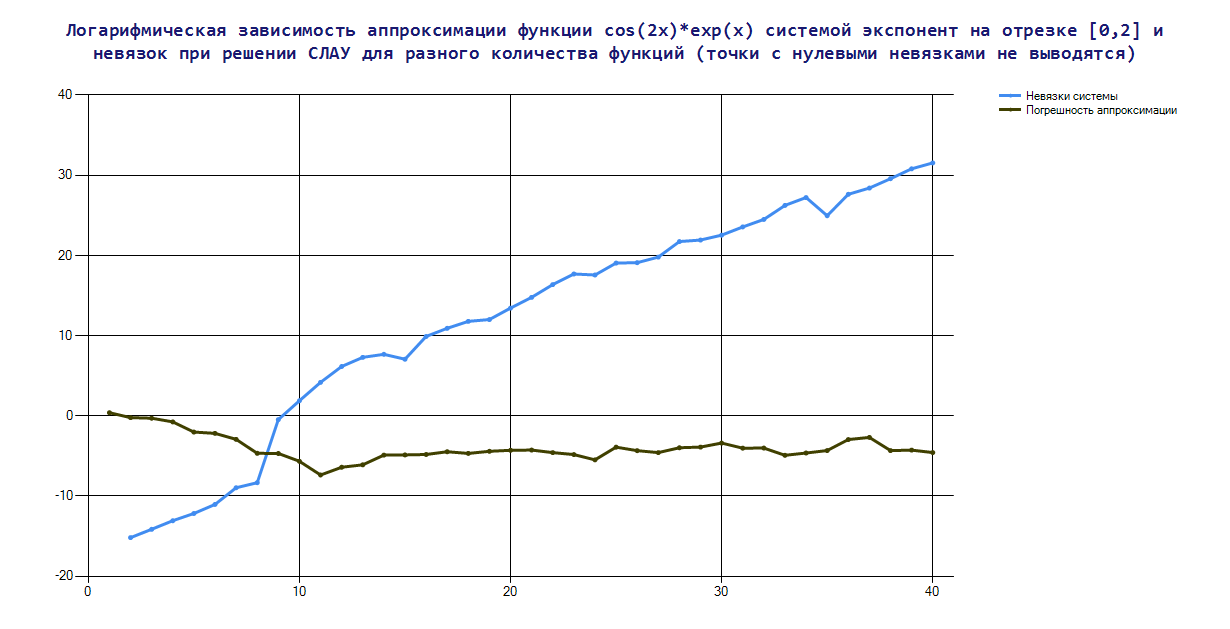
\includegraphics[width=\linewidth]{11.png}
  }
   \caption{Рост невязки не ведёт к увеличению погрешности}
    \label{figCurves}
\end{figure}

Следовательно, даже весьма неточное решение СЛАУ способно обеспечить относительно хорошую аппроксимацию. Вдобавок можно сделать вывод, что даже при максимально точном решении СЛАУ в пределах машинных возможностей минимизация функции
\begin{equation}F\left(c\right)={\left\|\varphi -\sum^N_{m=1}{c_m}{\alpha }_m\right\|}_{{\ L}_2\left(Q\right)}\\\end{equation} 
даёт сбои, поскольку результаты тестирования показывают, что при многих значениях $M<N$ имеет место неравенство
\begin{equation}{\left\|\varphi -\sum^M_{m=1}{c_m}{\alpha }_m\right\|}_{{\ L}_2\left(Q\right)}<{\left\|\varphi -\sum^{M+1}_{m=1}{c_m}{\alpha }_m\right\|}_{{\ L}_2\left(Q\right)},\end{equation} 
хотя вполне очевиден другой набор коэффициентов $c_m,m=1,\ 2,\dots ,M+1$, обеспечивающий аппроксимацию лучше того набора, который находится программой, а именно:
\begin{equation}{\left\|\varphi -\sum^M_{m=1}{c_m}{\alpha }_m-{0\times \alpha }_{M+1}\right\|}_{{\ L}_2\left(Q\right)}={\left\|\varphi -\sum^M_{m=1}{c_m}{\alpha }_m\right\|}_{{\ L}_2\left(Q\right)}<{\left\|\varphi -\sum^{M+1}_{m=1}{c_m}{\alpha }_m\right\|}_{{\ L}_2\left(\partial Q\right)}.\end{equation} 

Значит, если при максимально возможном точном решении СЛАУ неустойчивость остаётся, то единственным оставшимся выходом для её устранения может быть только варьирование получившихся коэффициентов в таком направлении, чтобы аппроксимация стала минимальной. Теория при этом говорит, что получившаяся последовательность приближений должна, по крайней мере, не возрастать.

Попробуем провести манипуляции с приближённым решением СЛАУ с целью приблизить его не к истинному решению СЛАУ, а к истинному решению задачи аппроксимации, используя метод покоординатной минимизации.

\section{Метод покоординатной минимизации и его возможная ограниченность вследствие ошибок округления}

Допустим, гибридным методом был найден набор чисел $c_m,m=1,\ 2,\dots ,N$, являющийся максимально точным решением получившейся СЛАУ; однако, в самом деле, этот набор не обязан обеспечивать максимально хорошую аппроксимацию не только из-за неизбежных неточностей при вычислении скалярных произведений (интегралов), но и из-за плохой обусловленности матрицы Грамма и ошибок округления. Повторюсь, что решение системы
\begin{equation}\left( \begin{array}{ccc}
{{({\alpha }_1,\alpha }_1)}_{{\ L}_2\left(Q\right)} & \cdots  & {{({\alpha }_1,\alpha }_N)}_{{\ L}_2\left(Q\right)} \\ 
\vdots  & \ddots  & \vdots  \\ 
{{({\alpha }_N,\alpha }_1)}_{{\ L}_2\left(Q\right)} & \cdots  & {{({\alpha }_N,\alpha }_N)}_{{\ L}_2\left(Q\right)} \end{array}
\right)\left( \begin{array}{c}
c_1 \\ 
\vdots  \\ 
c_N \end{array}
\right)=\left( \begin{array}{c}
{\left(\varphi ,{\alpha }_1\right)}_{{\ L}_2\left(Q\right)} \\ 
\vdots  \\ 
{\left(\varphi ,{\alpha }_N\right)}_{{\ L}_2\left(Q\right)} \end{array}
\right)\\\end{equation} 
является максимально точным, но сама система лишь приближённо является той, какой должна быть, вдобавок невязка такой системы существенно растёт с увеличением размерности. Отсюда можно сделать выводы, что некоторая корректировка набора $c_m,m=1,\ 2,\dots ,N$ оказывается не только полезной, но и обязательной, если при аппроксимации требуется добиться максимальной точности и устойчивости; это понятно и из вывода, сделанного в предыдущем пункте. Можно осуществить такую корректировку при помощи метода покоординатного спуска, который состоит в следующем (\cite{12sch,15lob}).

Найденный (любым методом) вектор $\left(c_1,c_2,\dots ,c_N\right)$ берётся за начальное приближение; после этого для каждого (либо для некоторых) $c_k,\ 1\le k\le N$ последовательно выполняется задача минимизации функции одной переменной
\begin{multline}
F\left(c_k\right)={\left\|\varphi -\sum^N_{m=1,m\neq k}{c_m}{\alpha }_m-{c_k\alpha }_k\right\|}_{{\ L}_2\left(\partial Q\right)}=\\
{\left(\varphi -\sum^N_{m=1,m\neq k}{c_m}{\alpha }_m-{c_k\alpha }_k,\varphi -\sum^N_{m=1,m\neq k}{c_m}{\alpha }_m-{c_k\alpha }_k\right)}^{\frac{1}{2}}_{{\ L}_2\left(\partial Q\right)}=\\
\Biggl(\left(\varphi ,\varphi \right)-2\sum^N_{m=1,m\neq k}{c_m}\left(\varphi ,{\alpha }_m\right)+\sum^N_{n=1,n\neq k}{c_n}\sum^N_{m=1,m\neq k}{c_m}{({\alpha }_n,\alpha }_m)+ \\
2\sum^N_{m=1,m\neq k}{c_m}c_k\left({\alpha }_k,{\alpha }_m\right)-2c_k\left({\alpha }_k,\varphi \right)+c^2_k\left({\alpha }_k,{\alpha }_k\right)\Biggl)^{\frac{1}{2}},
\end{multline} 
при этом полученный в конце новый вектор $\left(c_1,c_2,\dots ,c_N\right)$ теоретически гарантировано обеспечит лучшую аппроксимацию, а потому и устойчивость (устранив «скачки»).

Итак, реализуем задачу минимизации функции
\begin{multline}{F\left(c_k\right)}^2=\left(\varphi ,\varphi \right)-2\sum^N_{m=1,m\neq k}{c_m}\left(\varphi ,{\alpha }_m\right)+\\
\sum^N_{n=1,n\neq k}{c_n}\sum^N_{m=1,m\neq k}{c_m}{({\alpha }_n,\alpha }_m)+\\
2\sum^N_{m=1,m\neq k}{c_m}c_k\left({\alpha }_k,{\alpha }_m\right)-2c_k\left({\alpha }_k,\varphi \right)+c^2_k\left({\alpha }_k,{\alpha }_k\right)\end{multline} 
(возведение в квадрат не повлияет на решения, поскольку функция принимает исключительно неотрицательные значения). Стационарные точки:
\begin{multline}D_{c_k}F\left(c_k\right)=0\leftrightarrow 2\sum^N_{m=1,m\neq k}{c_m}\left({\alpha }_k,{\alpha }_m\right)-2\left({\alpha }_k,\varphi \right)+2c_k\left({\alpha }_k,{\alpha }_k\right)=0\to\\
c_k=\frac{\left({\alpha }_k,\varphi \right)-\sum^N_{m=1,m\neq k}{c_m}\left({\alpha }_k,{\alpha }_m\right)}{\left({\alpha }_k,{\alpha }_k\right)}.\end{multline} 
Очевидно, что найденная стационарная точка является точкой минимума, поскольку при переходе через неё производная функции меняет знак с отрицательного на положительный
\begin{equation}D_{c_k}F\left(c_k\pm \varepsilon \right)=2\sum^N_{m=1,m\neq k}{c_m}\left({\alpha }_k,{\alpha }_m\right)-2\left({\alpha }_k,\varphi \right)+2\left(c_k\pm \varepsilon \right)\times \left({\alpha }_k,{\alpha }_k\right)=\pm 2\varepsilon \left({\alpha }_k,{\alpha }_k\right)=\pm \omega ,\omega >0.\end{equation} 

При тестировании метода покоординатного спуска выяснилось, что он хорошо дополняет предыдущие методы, но его использование вовсе необязательно минимизирует функцию, если в точке начального приближения её значения уже достаточно близки к нулю. Иными словами, если за начальное приближение взять результат работы какого-либо предыдущего метода (то есть вектор $\left(c_1,c_2,\dots ,c_N\right)$ такой, что $0<F\left(c\right)\le \varepsilon $), то для получающегося вектора $\tau =\left({\tau }_1,{\tau }_2,\dots ,{\tau }_N\right)$ вовсе не обязательно будет выполняться $0<F\left(\tau \right)\le F\left(c\right)$, даже после многократного применения метода покоординатной минимизации; иногда, впрочем, случается, что $F\left(\tau \right)\le F\left(c\right)$, но при этом не никакой речи о каком-то монотонном улучшении качества аппроксимации не идёт, откуда и не получится устойчивости. Покажем основные результаты; во всех следующих примерах минимизация проводится по всем элементам вектора $c$ по 10 раз.

Неустойчивость (Рис. 14).

\begin{figure}[h!]
    \noindent\centering{
    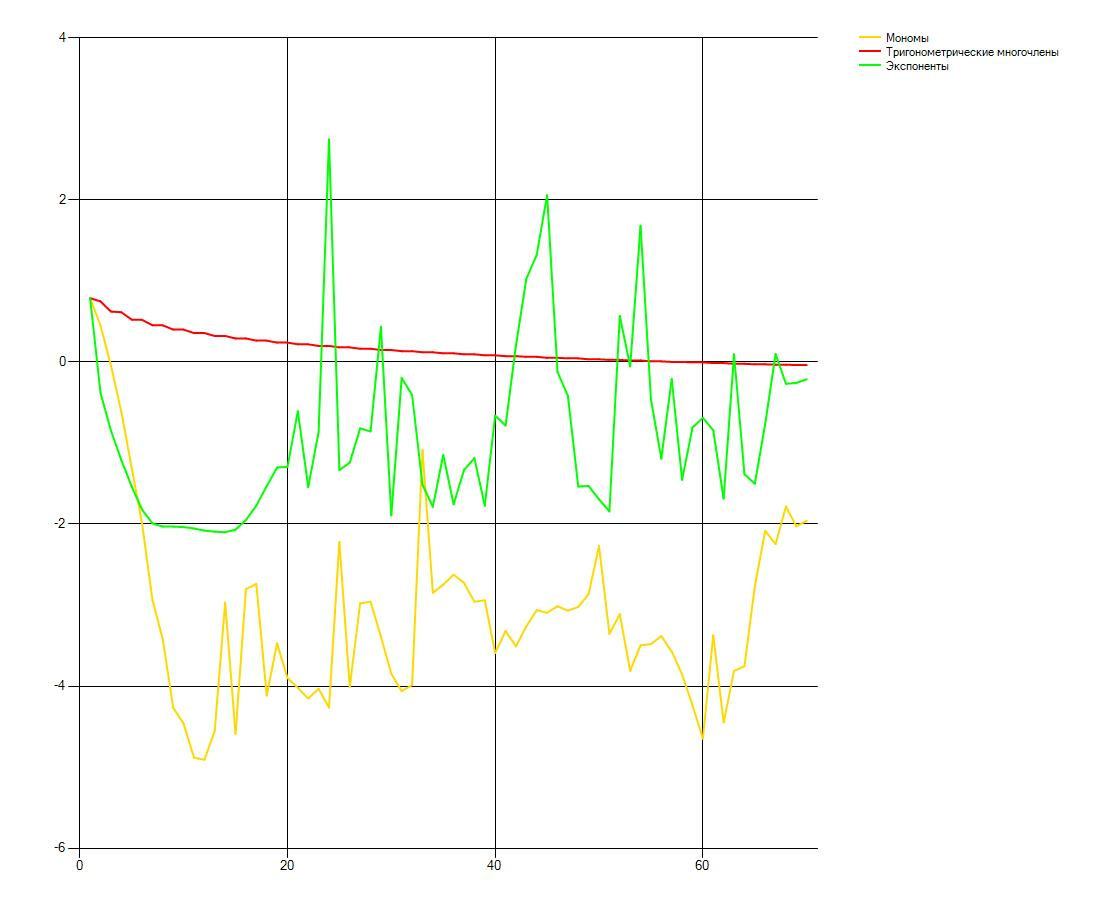
\includegraphics[width=\linewidth]{12.png}
  }
   \caption{Неустойчивая аппроксимация методом покоординатной минимизации}
    \label{figCurves}
\end{figure}

Погрешность и невязка в зависимости от числа функций (Рис. 13).

\begin{figure}[h!]
    \noindent\centering{
    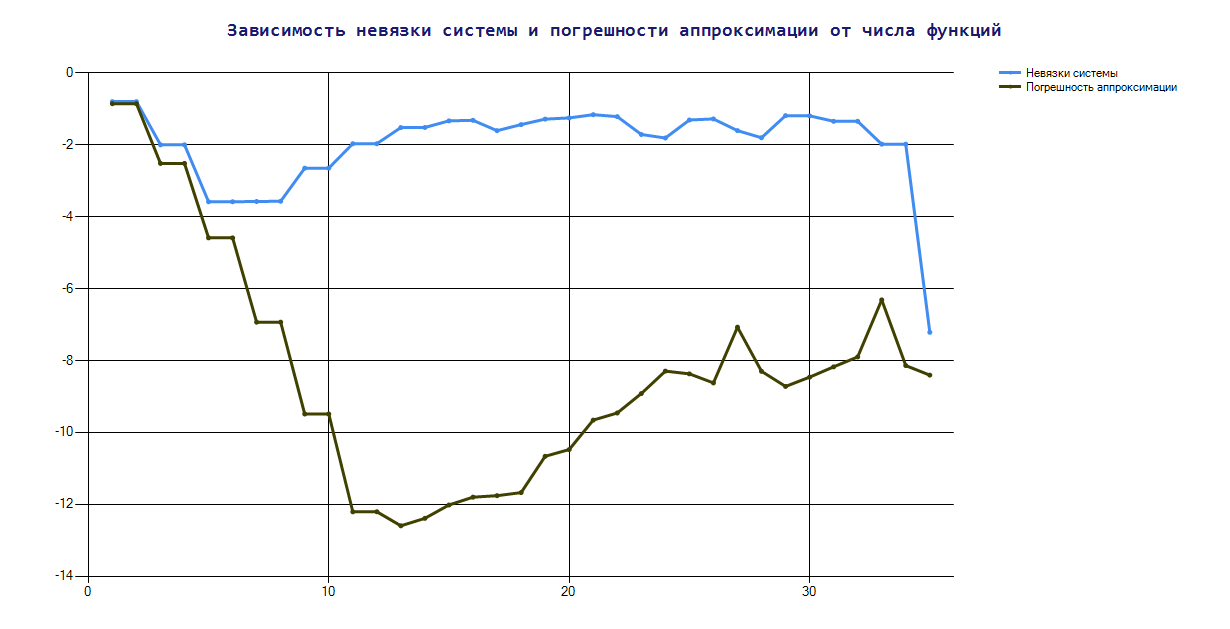
\includegraphics[width=\linewidth]{121.png}
  }
   \caption{Зависимость невязки системы и погрешности аппроксимации от числа функций, используется система мономов на отрезке $[-1;1]$, система решается гибридным методом с последующей покоординатной минимизацией}
    \label{figCurves}
\end{figure}

В этом же примере при любом числе функций многократная минимизация стабильно действует, хоть и очень медленно (Рис. 16).

\begin{figure}[h!]
    \noindent\centering{
    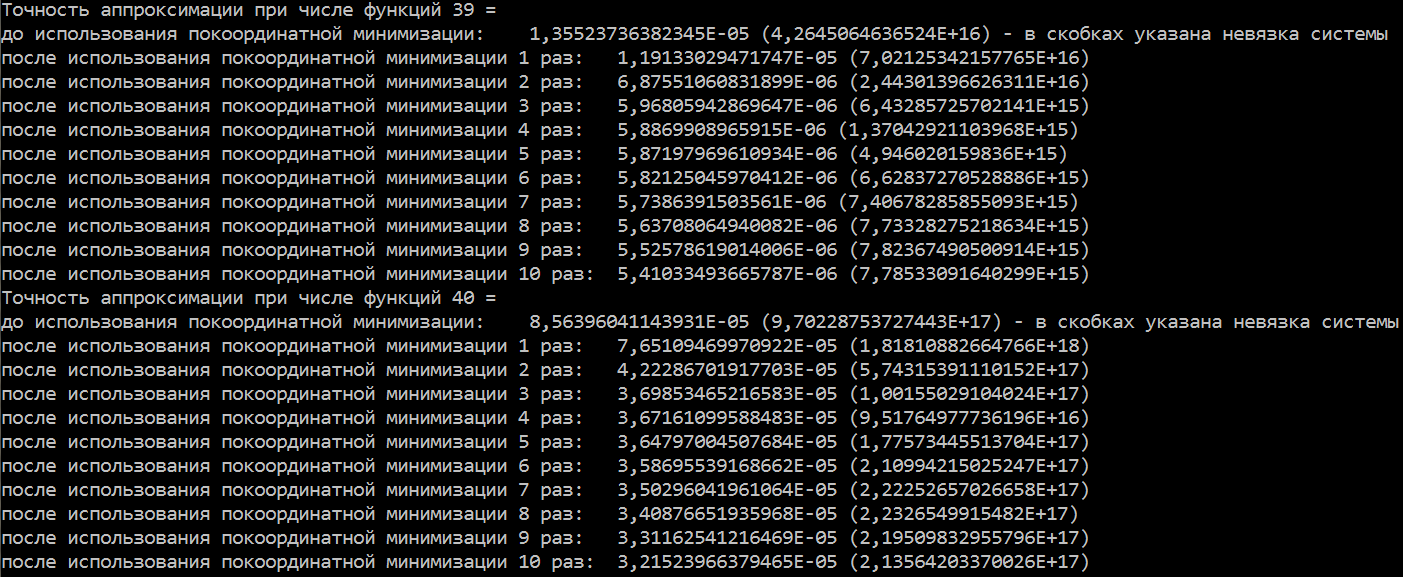
\includegraphics[width=\linewidth]{13.png}
  }
   \caption{Многократная минимизация медленно уточняет решение}
    \label{figCurves}
\end{figure}

Как видно из предыдущих графиков, уменьшение погрешности аппроксимации не обязательно уменьшает невязку. В данном случае погрешность стабильно уменьшается, однако часто она может возрастать при использовании покоординатной минимизации при решении достаточно сложных задач аппроксимации. В следующем примере происходит аппроксимация функции двух переменных, заданной на окружности, по системе логарифмов (базисных потенциалов)
\begin{equation}{\alpha }_m\left(y\right)={\mathrm{ln} \frac{1}{\left|z^m-y\right|}={\mathrm{ln} \frac{1}{\sqrt{\sum^{\mathrm{2}\ }_{n=1}{{\left(z^m_n-y_n\right)}^2}}}\ },\ }\ z^m\in Q^+,\ m=1,\ 2,\ \dots ,\ y\in \partial Q,\\\end{equation} 
где  $\partial Q$ -- граница круга (окружность, на которой ведётся аппроксимация), $Q^+$-- внешность круга, $z^m$ -- некоторый набор точек, удовлетворяющий определённым условиям. В этом случае при достаточно большом числе функций многократное использования покоординатной минимизации не только не обеспечивает монотонное убывание, но и само убывание не гарантирует (Рис. 17).

\begin{figure}[h!]
    \noindent\centering{
    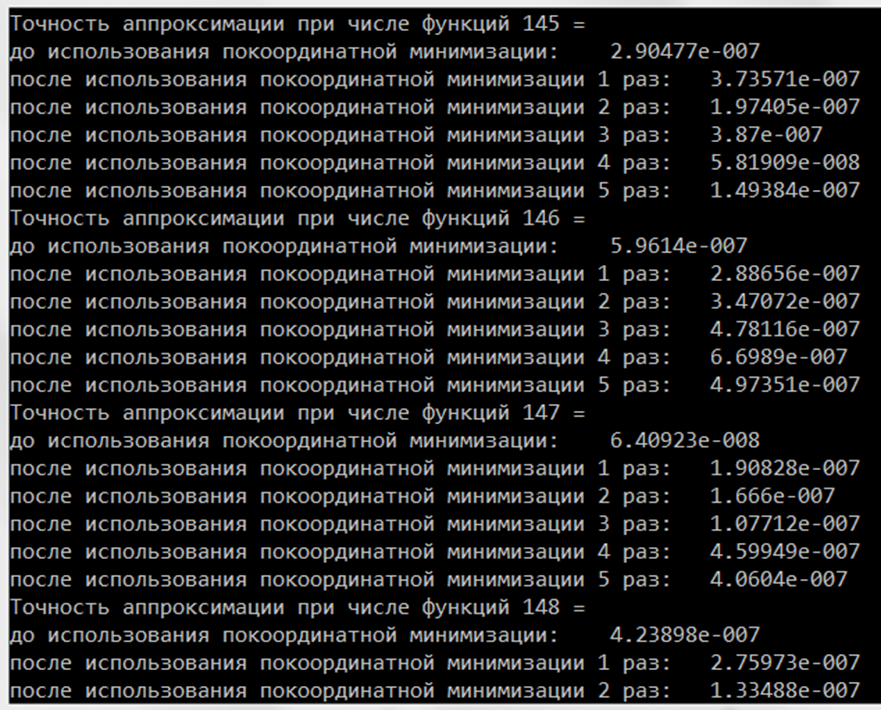
\includegraphics[width=13cm]{14.png}
  }
   \caption{Многократная минимизация не обязательно уточняет решение}
    \label{figCurves}
\end{figure}

Тесты, подобные предыдущему, привели к предположению, что метод покоординатной минимизации не способен гарантированно уменьшать погрешность аппроксимации ниже некоторого фиксированного значения, определённого условиями задачи. При простейшей аппроксимации функции на отрезке погрешность в подавляющем большинстве тестов убывала гарантированно, хоть и медленно; может быть, вероятность неубывания погрешности тем больше, чем меньше невязка системы, что видно из следующего случая (Рис. 18). 

\begin{figure}[h!]
    \noindent\centering{
    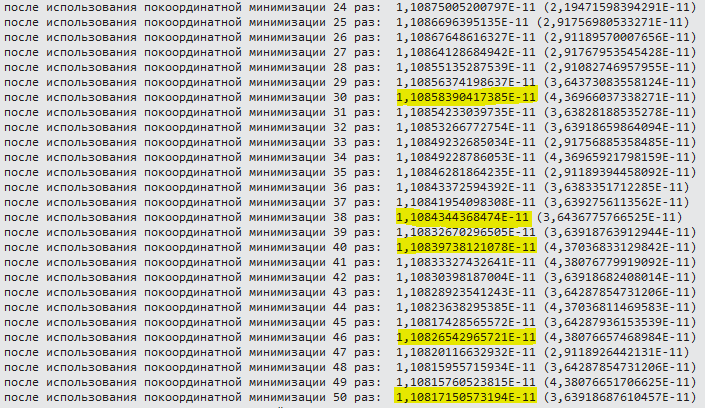
\includegraphics[width=13cm]{15.png}
  }
   \caption{Негарантированное убывание погрешности при многократном использовании метода покоординатной минимизации для аппроксимации функции $y=x^3-x+4$ системой мономов на отрезке от 0 до 5}
    \label{figCurves}
\end{figure}

Зафиксируем промежуточные выводы:
\begin{enumerate}
\item  Решение задачи аппроксимации классическими алгоритмами получается неустойчивым вследствие погрешностей квадратур, плохой обусловленности матриц Грама и ошибок округления.

\item  Увеличение точности интегрирования безусловно «сглаживает» неустойчивость, однако считать интегралы идеально точно нельзя, поэтому в подсчёте интегралов требуется достигнуть компромисса между точностью и быстродействием, а избавляться от неустойчивости требуется независимо от точности интегрирования.

\item  Классический и модифицированный методы Гаусса не способны точно решать плохо обусловленные СЛАУ большой размерности. Поскольку при большой (от 12-15) размерности матрица Грама перестаёт быть численно положительно определённой, метод Холецкого на большой размерности работать не может, а метод наискорейшего спуска чаще всего расходится. Решая СЛАУ, можно найти лишь приближённое решение, которое придётся как-нибудь модифицировать с целью уменьшить погрешность аппроксимации, а не невязку.

\item  Метод покоординатной минимизации почти гарантирует убывание погрешности аппроксимации, пусть медленное. Его можно использовать для улучшения аппроксимации при конкретном числе функций, но устойчивости от также не гарантирует. Возможно, устойчивый алгоритм не может не быть многошаговым.
\end{enumerate}

\section{Многошаговый алгоритм аппроксимации, гарантирующий устойчивость}

Модификация и слияние нескольких описанных ранее методов, а также учёт некоторых замечаний, привели к созданию устойчивого многошагового алгоритма решения задачи аппроксимации; он никак не привязан к какой-либо системе функций и должен эффективно работать для любой линейно независимой системы. Назовём этот метод {\it ультра-гибридным}. Вот в чём он заключается.

Допустим, требуется минимизировать функционал
\begin{equation}F\left(c^M\right)={\left\|\varphi -\sum^M_{m=1}{c_m}{\alpha }_m\right\|}_{{\ L}_2\left(\partial Q\right)},\end{equation} 
причём его минимизация должна удовлетворять условию
\begin{equation}F\left(c^{M-1}\right)\ge F\left(c^M\right)\ge F\left(c^{M+1}\right),\ M\ge 2.\end{equation} 
Такую минимизацию можно осуществить по индукции:

Если $M=1$, решение очевидно: $c_1=\left({\alpha }_1,\varphi \right)/\left({\alpha }_1,{\alpha }_1\right)$. В противном случае требуется искать решения для $c^2$, $c^3$,{\dots}, $c^{M-1}$ последовательно; допустим, они найдены, тогда:

Шаг 1 (СПИДГАУСС). Найти вектор $c^M=\left(c_1,c_2,\dots ,c_M\right)$, решив известную СЛАУ описанным ранее гибридным методом (либо любым другим).

Шаг 2 (МИНИМАКА СПИДГАУССА). Если $F\left(c^{M-1}\right)<F\left(c^M\right)$, то применить ко всем компонентам $c^M$покоординатную минимизацию (возможно, несколько раз).

Шаг 3 (ПОЛНАЯ МИНИМАКА). Если снова $F\left(c^{M-1}\right)<F\left(c^M\right)$, то вектор $c^M$ заменить на вектор $\left(c^{M-1}_1,c^{M-1}_2,\dots ,c^{M-1}_{M-1},0\right)$ и провести покоординатную минимизацию по всем компонентам этого вектора.

Шаг 4 (МИНИМАКА НА КОНЦЕ). Если снова $F\left(c^{M-1}\right)<F\left(c^M\right)$, то вектор $c^M$ снова заменить на вектор $\left(c^{M-1}_1,c^{M-1}_2,\dots ,c^{M-1}_{M-1},0\right)$ и применить покоординатную минимизацию только для последнего элемента
\begin{equation}c^M=\left(c^{M-1}_1,c^{M-1}_2,\dots ,c^{M-1}_{M-1},\frac{\left({\alpha }_M,\varphi \right)-\sum^{M-1}_{m=1}{c_m}\left({\alpha }_M,{\alpha }_m\right)}{\left({\alpha }_M,{\alpha }_M\right)}\right).\end{equation} 

Шаг 5. Если и в таком случае $F\left(c^{M-1}\right)<F\left(c^M\right)$, то 
\begin{equation}c^M=\left(c^{M-1}_1,c^{M-1}_2,\dots ,c^{M-1}_{M-1},0\right)\to F\left(c^{M-1}\right)=F\left(c^M\right).\end{equation} 

Аппроксимативные свойства этого метода, очевидно, не хуже, чем у гибридного; при этом устойчивость гарантирована. Практика показывает, что шаги 1-4 не являются равнозначными и в каждом конкретном случае любой из них может уменьшить погрешность аппроксимации там, где остальные не могут.

Следующие графики (Рис. 19-24) показывают, насколько метод устойчив; обратите внимание, что зачастую ультра-гибрид позволяет аппроксимировать не только устойчиво, но и точнее любого другого метода (кривая ультра-гибрида опускается ниже минимального значения для другого метода).

\begin{figure}[h!]
    \noindent\centering{
    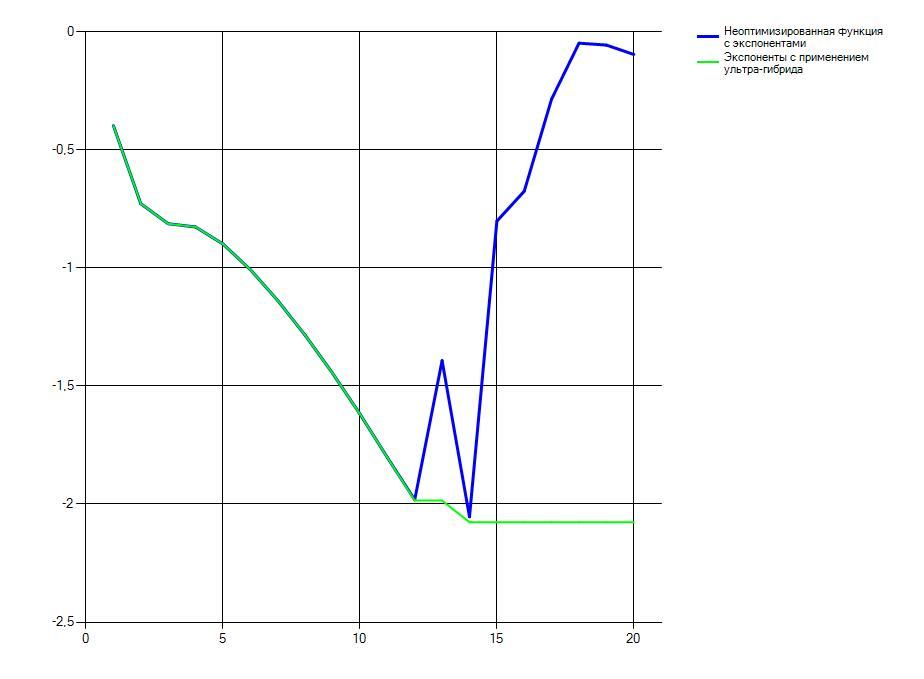
\includegraphics[width=\linewidth]{16.png}
  }
   \caption{Устойчивая аппроксимация экспонентами с помощью ультра-гибрида}
    \label{figCurves}
\end{figure} 

\begin{figure}[h!]
    \noindent\centering{
    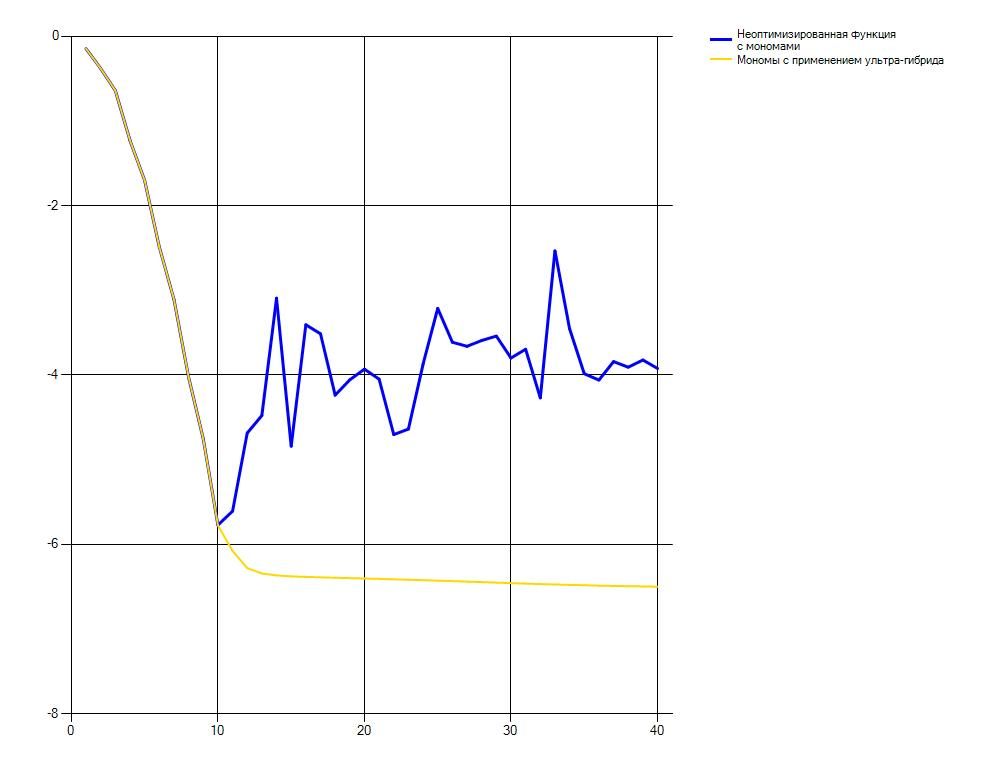
\includegraphics[width=\linewidth]{17.png}
  }
   \caption{Устойчивая аппроксимация мономами с помощью ультра-гибрида}
    \label{figCurves}
\end{figure}

\begin{figure}[h!]
    \noindent\centering{
    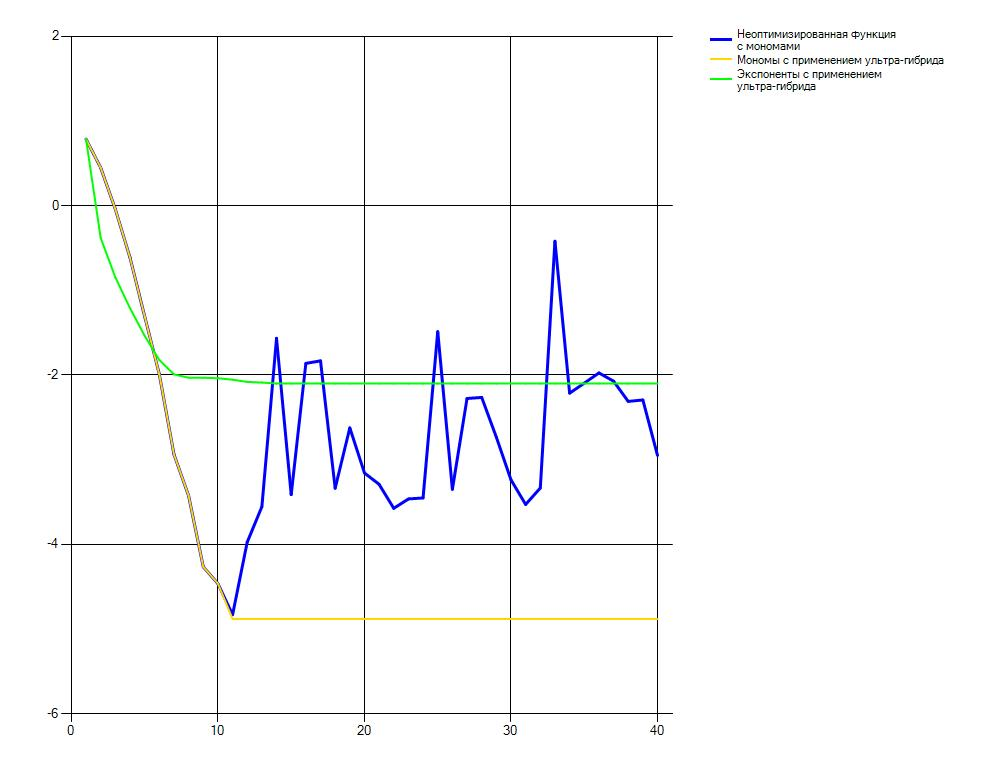
\includegraphics[width=\linewidth]{18.png}
  }
   \caption{Устойчивая аппроксимация экспонентами и мономами с помощью ультра-гибрида}
    \label{figCurves}
\end{figure}

Ультра-гибрид исправляет в том числе неустойчивость аппроксимации по ортогональным функциям (Рис. 22-23).

\begin{figure}[h!]
    \noindent\centering{
    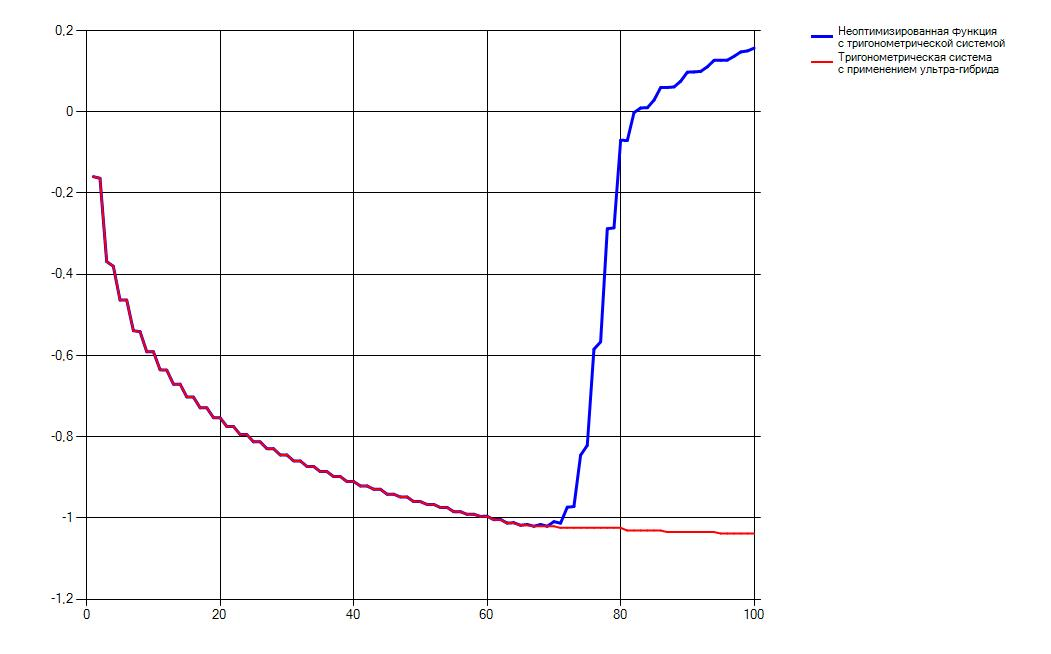
\includegraphics[width=\linewidth]{19.png}
  }
   \caption{Устойчивая аппроксимация системой синусов и косинусов с помощью ультра-гибрида}
    \label{figCurves}
\end{figure}

\begin{figure}[h!]
    \noindent\centering{
    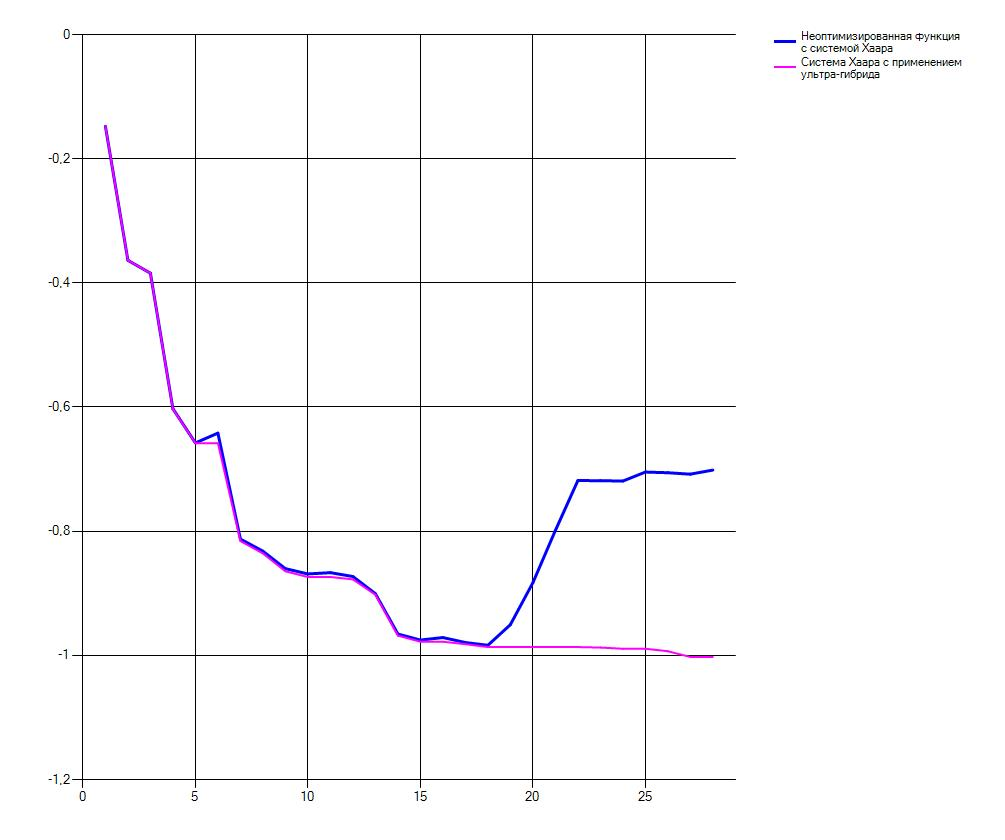
\includegraphics[width=\linewidth]{20.png}
  }
   \caption{Устойчивая аппроксимация системой Хаара с помощью ультра-гибрида}
    \label{figCurves}
\end{figure}

А вот так метод «выглядит изнутри» (Рис. 24).

\begin{figure}[h!]
    \noindent\centering{
    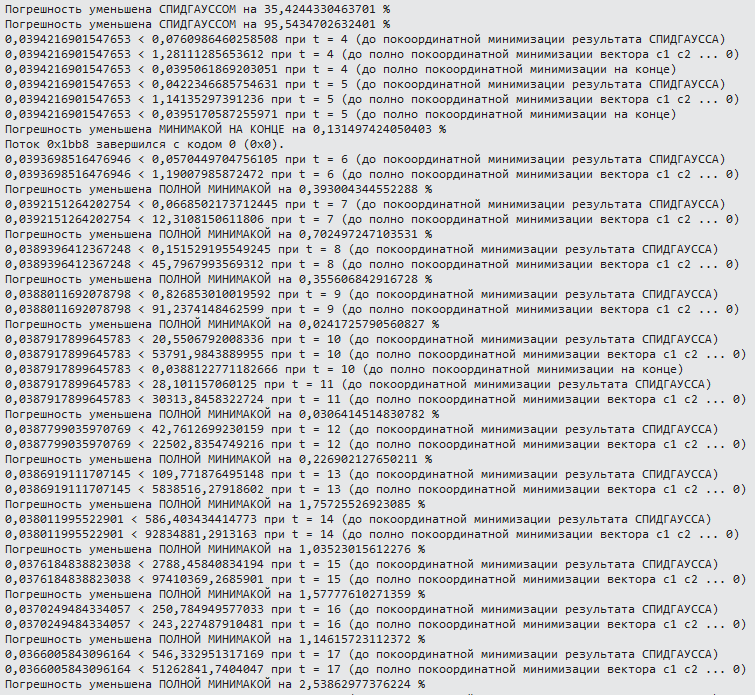
\includegraphics[width=\linewidth]{21.png}
  }
   \caption{Как с помощью ультра-гибрида происходит уточнение решения. В неравенствах слева указана наилучшая достигнутая на данный момент аппроксимация, справа -- достигнутая на текущей итерации при текущем шаге, $t$ -- количество функций на текущей итерации. Как видно, на отдельных шагах аппроксимация может существенно возрастать, иногда ни один из шагов не даёт результата в нескольких итерациях, однако раз в несколько итераций аппроксимация улучшается каким-либо отдельным методом и в общем происходит убывание погрешности}
    \label{figCurves}
\end{figure}

\section{Замечание об ортогональных системах}

Известно, что для ортогональных систем матрица Грама диагональна, поэтому проекция аппроксимируемой функции на исходное подпространство выражается аналитически рядом Фурье и тогда:
\begin{equation}{\left\|\varphi -\sum^N_{m=1}{c_m}{\alpha }_m\right\|}_{{\ L}_2\left(Q\right)}={\left\|\varphi -\sum^N_{m=1}{\left(\varphi ,{\alpha }_m\right)/{({\alpha }_m,\alpha }_m)}{\alpha }_m\right\|}_{{\ L}_2\left(Q\right)}=\mathrm{min}.\end{equation}

Поэтому рекомендуется по возможности использовать ортогональные системы, чтобы минимизировать время вычислений и погрешности. Ранее было показано, что такая аппроксимация убывает очень медленно и не застрахована от неустойчивости. Также было показано, что в свете этого зачастую эффективнее аппроксимировать по неортогональной системе небольшой размерности (пусть даже по неустойчивому алгоритму), чем вычислять решение в виде ряда $\sum^N_{m=1}{\left(\varphi ,{\alpha }_m\right)/{({\alpha }_m,\alpha }_m)}{\alpha }_m$ по нескольким сотням функций. Не в пользу одного из методов говорят и новые данные: в ходе тестирования ультра-гибридного метода было обнаружено, что между записью решения в виде ряда $\sum^N_{m=1}{\left(\varphi ,{\alpha }_m\right)/{({\alpha }_m,\alpha }_m)}{\alpha }_m$ и решением диагональной СЛАУ, соответствующей этому ряду, на практике существует разница: по неизвестным причинам решение задачи аппроксимации для ортогональных систем иногда становится точнее, если решать её описанным выше традиционным методом (через решение СЛАУ), не обращая внимания на то, что в теории решение можно записать сразу же; кроме того, убывание погрешности происходит быстрее, а неустойчивость менее выражена. Следующие графики (Рис. 25-26) это подтверждают; в обоих случаях аппроксимация происходит по неустойчивому алгоритму для небольшого числа функций, потому что цель -- показать разницу двух способов решения одной и той же задачи; графики представлены для системы Хаара, на которой это явление и было замечено; с тригонометрической системой этот способ работает в точности наоборот; к слову, попытки ускорить вычисления многочленов Лежандра ранее привели к усиленной неустойчивости, так что описанное явление явно связано с погрешностями вычислений. 

\begin{figure}[h!]
    \noindent\centering{
    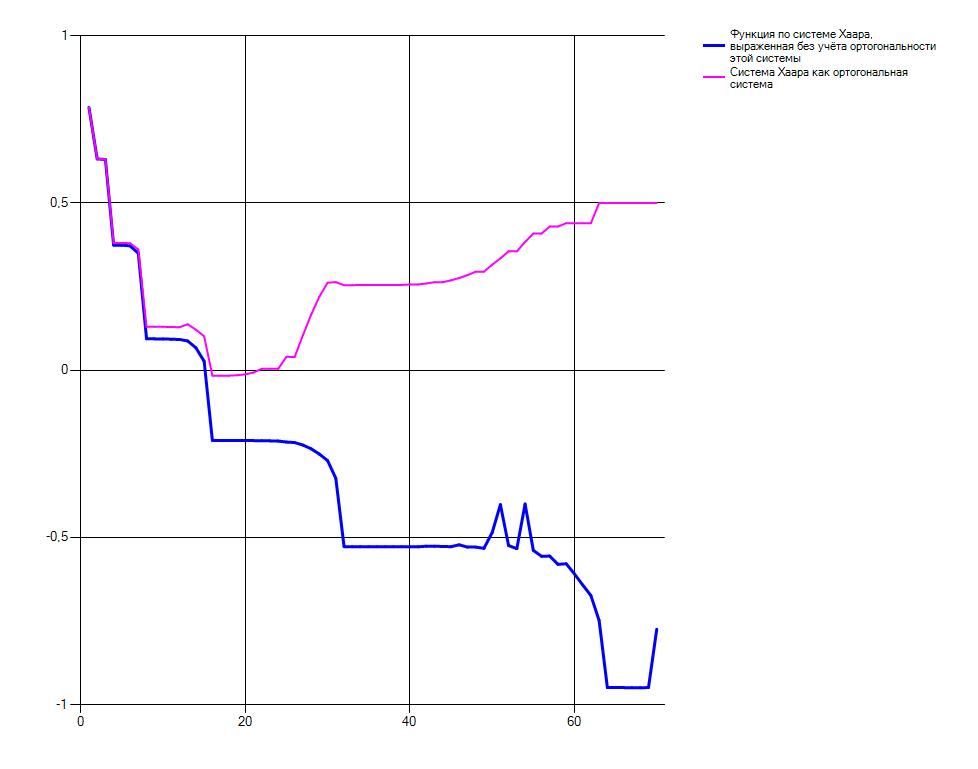
\includegraphics[width=\linewidth]{22.png}
  }
   \caption{Разница между двумя способами аппроксимации системой Хаара}
    \label{figCurves}
\end{figure}

\begin{figure}[h!]
    \noindent\centering{
    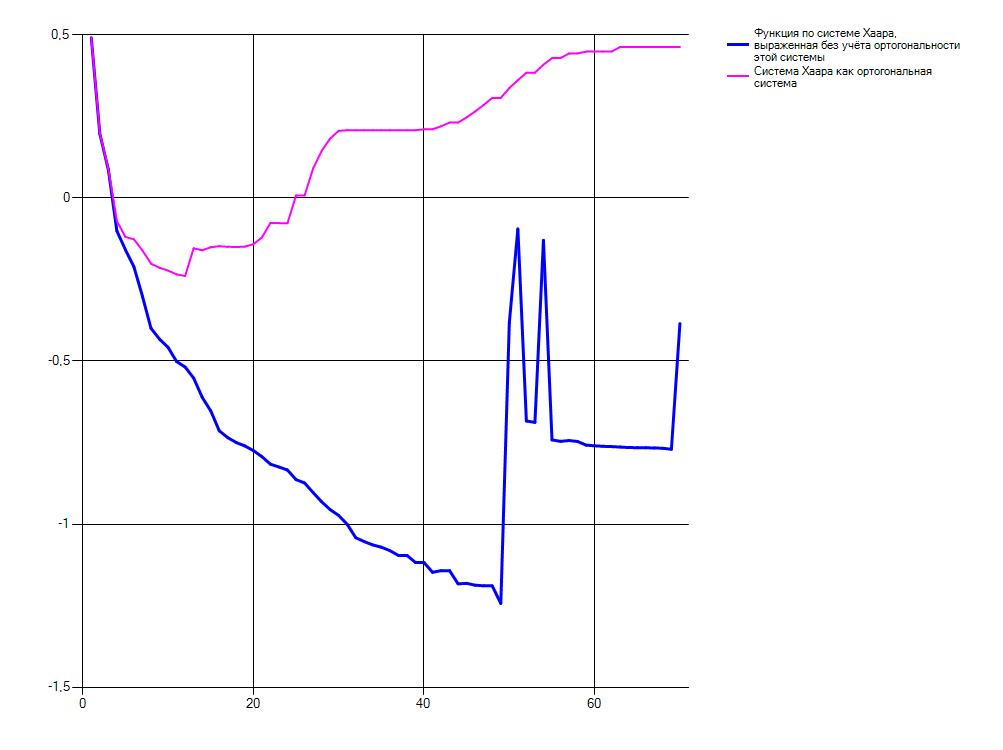
\includegraphics[width=\linewidth]{23.png}
  }
   \caption{Такая же разница при других начальных данных задачи}
    \label{figCurves}
\end{figure}

\section{Примеры использования ультра-гибридного метода для аппроксимации в пространствах, отличных от $L_2[a,b]$ }

При практических расчётах аппроксимируемая функция обычно известна либо по набору значений (причём приближённых), либо по своему образу, полученному через дифференциальный или интегральный оператор. Рассмотрим, какую пользу приносит ультра-гибридный метод при решении таких задач на примере МНК и обратной задачи потенциала.

В методе наименьших квадратов происходит дискретное среднеквадратическое приближение сеточной функции, заданной в $n$ точках, измеримыми функциями. В таком случае выкладки получаются абсолютно такими же, как при аппроксимации в ${\ L}_2\left(Q\right)$, но используются другие выражения для скалярного произведения
\begin{equation}{\left(f,\varphi \right)}_{R^{\left[a,b\right]}_n}=\frac{1}{n}\sum^n_{i=1}{f\left(x_i\right)\varphi \left(x_i\right)}\\\end{equation} 
и нормы
\begin{equation}{\left\|f\right\|}_{R^{\left[a,b\right]}_n}=\sqrt{\frac{1}{n}\sum^n_{i=1}{f{\left(x_i\right)}^2}}.\end{equation} 
Несмотря на более точное вычисление скалярных произведений в случае сеточной функции, в МНК так же встречается неустойчивость. Аппроксимируем, например, фиксированную сеточную функцию (проекцию действительной функции) некоторыми системами размерности 4 (Рис. 27).

\begin{figure}[h!]
    \noindent\centering{
    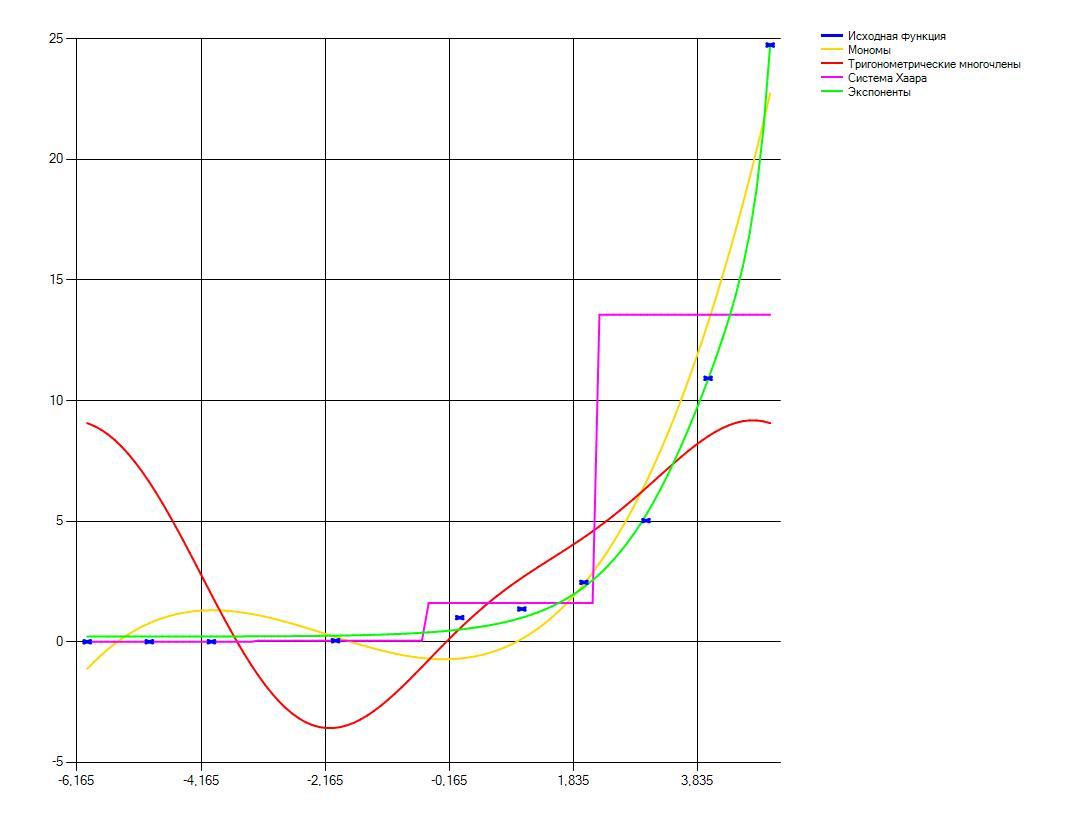
\includegraphics[width=\linewidth]{24.png}
  }
   \caption{Аппроксимация сеточной функции несколькими системами размерности 4}
    \label{figCurves}
\end{figure}

Качество аппроксимации для системы Хаара следующее: в интегральной среднеквадратичной норме равна 3,41841902293629, в равномерной норме равна 11,1746183943873, в дискретной среднеквадратичной норме равна 4,53800130664926. Если увеличить количество функций до 6, получим заметную неустойчивость (Рис. 28). 

\begin{figure}[h!]
    \noindent\centering{
    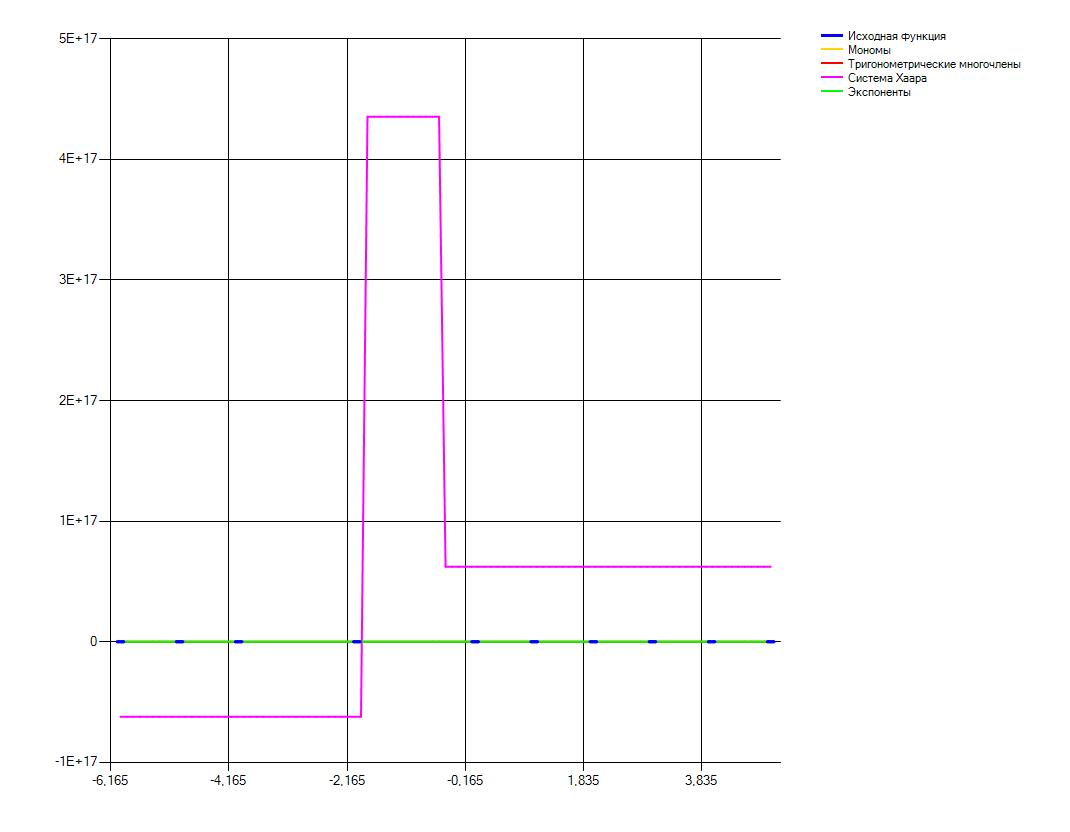
\includegraphics[width=\linewidth]{25.png}
  }
   \caption{Неустойчивость системы Хаара при размерности 6}
    \label{figCurves}
\end{figure}

Те же данные об аппроксимации: погрешность аппроксимации в интегральной среднеквадратичной норме равна 1,50959632325169E+17, в равномерной норме равна 4,35248462504321E+17, в дискретной среднеквадратичной норме) равна 6,21783517863316E+16.



\section{Обзор результатов}


\begin{thebibliography}{999} 
    \bibitem{5alg}
    С. Дасгупта, Х. Пападимитриу, У. Вазирани. Алгоритмы.~---
    М.: МЦНМО, 2014.
    \bibitem{8kol}
    Колмогоров А. Н., Фомин С. В.. Элементы теории функции и функционального анализа.~---
    М.: Наука. Гл. ред. физ.-мат. лит. 1989.
    \bibitem{9korn}
    Н. П. Корнейчук. Экстремальные задачи теории приближения.~---
    М.: Наука. Гл. ред. физ.-мат. лит. 1976.
    \bibitem{10ax}
    Н. И. Ахиезер. Лекции по теории аппроксимации.~---
    М.: Наука. Гл. ред. физ.-мат. лит. 1964.
    \bibitem{12sch}
    Г. С. Шевцов, О. Г. Крюкова, Б. И. Мызникова. Численные методы линейной алгебры: Учеб. пособие.~---
    М.: Финансы и статистика: ИНФРА-М, 2008.
    \bibitem{15lob}
    И. Б. Петров, А. И. Лобанов.. Лекции по вычислительной математике: Учебное пособие.~---
    М.: Интернет-Университет Информационных Технологий; БИНОМ. Лабиринт знаний, 2006.
    \bibitem{algol}
    Справочник алгоритмов на языке АЛГОЛ. Линейная алгебра.~---
    М.: Машиностроение, 1976.
\end{thebibliography}

\end{document}

